\documentclass[a4paper, 11pt, twoside]{article}

\usepackage{hyperref}
%\usepackage[ngerman]{babel}
\usepackage[english]{babel}
%\usepackage[latin1]{inputenc}
\usepackage[utf8]{inputenc}

\usepackage{graphicx,float,subfigure}
%\usepackage{pifont}
\usepackage{type1cm}
\usepackage{amssymb, amsthm, amsmath,amsbsy}
\usepackage{listings}
\usepackage{graphicx}
\usepackage{subfigure}
\usepackage{xcolor}
\usepackage{tabularx}
\usepackage{tikz}
\tikzset{every path/.append style={line width=1pt}}
\usepackage{pgfplots}
\pgfplotsset{compat=newest} % Allows to place the legend below plot
\usetikzlibrary{positioning, decorations.pathreplacing,decorations.markings}
\definecolor{unirot}{rgb}{0.5976525,0,0}
\usepackage{pgf}
\usepackage{url}
%\usepackage{graphicx}
%\usepackage{pifont}
%\usepackage{type1cm}


\usepackage{makeidx}
\makeindex

\setlength{\parindent}{0em}
\setlength{\oddsidemargin}{0.0cm}
\setlength{\evensidemargin}{0.0cm}
\setlength{\textheight}{23cm}
\setlength{\topmargin}{-0.5cm}
\setlength{\footskip}{1.5cm}
\setlength{\textwidth}{15.5cm}

\renewcommand*\familydefault{\sfdefault}

\begin{document}
\thispagestyle{empty}

\include{frontpage_hiflow_poisson_adaptive_tutorial}

%\newpage
%\null\newpage

\newcommand{\dd}{\mathrm{d}}
\newtheorem{remark}{Remark}[section]
\thispagestyle{empty}
\tableofcontents

\newpage
\pagestyle{plain}
\framebox[15.5cm]{\parbox[c][2.3cm]{14.0cm}{
{\fontsize{19}{30}\selectfont{} \bf{ Error Estimation on Convex Bent Domains\\[0.5em] for the Poisson Equation}
}}}
\vspace{0.5cm}
\section{Introduction}

HiFlow$^3$ is a multi-purpose Finite Element software providing powerful tools for efficient and accurate solution of a wide range of problems modeled by partial differential equations (PDEs). Based on object-oriented concepts and the full capabilities of C++ the HiFlow$^3$ project follows a modular and generic approach for building efficient parallel numerical solvers. It provides highly capable modules dealing with the mesh setup, Finite Element spaces, degrees of freedom, linear algebra routines, numerical solvers, and output data for visualization. Parallelism - as the basis for high performance simulations on modern computing systems - is introduced on two levels: coarse-grained parallelism by means of distributed grids and distributed data structures, and fine-grained parallelism by means of platform-optimized linear algebra back-ends.

\subsection{How to Use the Tutorial?}
You find the example code (poisson\_adaptive.cc, poisson\_adaptive.h) and a parameter file for the first numerical example (poisson\_adaptive.xml) in the folder \verb'/hiflow/examples/poisson'. The geometry data (*.inp, *.vtu) is stored in the folder \verb'/hiflow/examples/data'.

\subsubsection{Using HiFlow$^3$ as a Developer}\label{sectiondeveloper}
First build and compile HiFlow$^3$. Go to the directory \verb'/build/example/poisson', where the binary \textbf{poisson\_adaptive} is stored. Type \textbf{./poisson\_adaptive}, to execute the program. 
You need to make sure that the default parameterfile poisson\_adaptive.xml is stored in the same directory as the binary, and that the geometry data specified in the parameter file is stored in \verb'/hiflow/examples/data'. Alternatively, you can specify the path of your own xml-file with the name of your xml-file (first) and the path of your geometry data (second) in the comment line, i.e. \textbf{./poisson\_adaptive} \verb'/"path_to_parameterfile"/"name_of_parameterfile".xml' \verb'/"path_to_geometry_data"/'.


\section{Mathematical Setup}
\subsection{Problem}
Note: For simplification, we explain the mathematical setup and the examples only for the two dimensional case. 
However, it is easy to extend the theory and the implementation to one or three dimensions.\\
Our aim is to solve the Poisson problem with a homogeneous Dirichlet boundary condition on a domain $\Omega \subset \mathbb{R}^2$ with sufficiently smooth but convexly or concavely
bent parts of the boundary $\partial \Omega$.
\begin{figure}[!htbp]
\centering
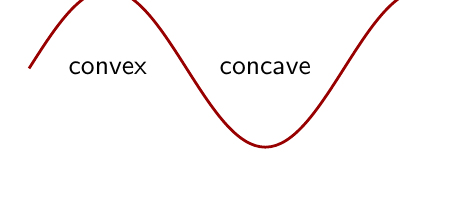
\begin{tikzpicture}
\draw[unirot] (0,0) sin(1,1) cos(2,0) sin(3,-1) cos(4,0) sin(5,1);
\draw (1,0) node {convex};
\draw (3,0) node {concave};
\end{tikzpicture}
\caption{convexly and concavely bent boundary}
\end{figure}
With this background we want to find a computable upper bound for the error of the Finite Element method on domains with bent boundaries.
As a next step we will test and evaluate the new constructed a-posteriori error estimator for domains with bent boundaries.
For given $f \in C(\Omega)$, the weak formulation of the Poisson problem
\begin{eqnarray}\label{poisson_equation}
\begin{array}{rcll}
-\Delta u &=& f, & \text{ in }\Omega,\\
        u &=& 0, & \text{ on }\partial\Omega,
\end{array}
\end{eqnarray}
is given by
\begin{align*}
 u \in V\qquad\ \ \	(\nabla u,\nabla \phi) =&\ (f,\phi)\ \qquad	\forall \phi \in V,\\
u_h \in V_h \subset V\qquad	(\nabla u_h,\nabla \phi_h) =&\ (f,\phi_h)\qquad	\forall \phi_h \in V_h.
\end{align*}
Here, $(\cdot,\cdot)$ is the $L^2$-scalar product on $\Omega$ or on the discrete ansatz space $\Omega_h$.
The Lax-Milgram theorem guarantees the existence of $u$ and $u_h$.

The solution $u_h$ resulting from the Finite Element method will be an approximation of the exact solution $u$. 
The error $(u-u_h)$ measures the quality of the discrete solution.
The natural error norm for a elliptic partial differential equation is the $H^1$-norm. 
For the sake of simplicity we will focus on the case of convex boundaries. However, 
it should be possible to construct an a-posteriori error estimator for domains with concavely bent boundaries as well by using similar methods. 
\subsection{A-posteriori error estimation}
Being defined locally, an a-posteriori error estimator provides information about where the biggest contributions to the error are to be expected.
As we are talking about an a-posteriori estimator it just should depend on the computable quantities $f$, $u_h$ and $\Omega_h$.
The standard residual based error estimator works well for domains with polygonal boundaries. \\

The following theory assumes that we discretize with a regular triangulation, where is $\Delta u_h|_T = 0$.
\subsubsection{The standard a-posteriori error estimator}\label{richterskript}
Under the assumption that  $u \in V$ fulfills the variational formulation of our problem and that $u_h \in V_h$ is the linear Finite Element approximation we know that 
the error $e_h:=u-u_h$ can be estimated by
\begin{eqnarray}
\| \nabla e_h\|_{L^2(\Omega)} \leq c\, \eta_h,\quad \eta_h := \left(\sum_{T \in \Omega_h}(\rho_T^2+ \sum_{E \in \partial T}\rho_E^2)\right)^{\frac{1}{2}}.\label{aposteriori}
\end{eqnarray}
Here, the cell residuals $\rho_T$ and the edge residuals $\rho_E$ are defined by
\begin{align*}
\rho_T&:=h_T\, \| f \|_{L^2(T)},\\
\rho_E&:=\frac{1}{2}\ h_E^{\frac{1}{2}}\, \|[n_E \cdot \nabla u_h]\|_{L^2(E)}.
\end{align*}
The notation $[,]$ refers to the jump over an inner edge between two neighbor cells $T_1$ and $T_2$, defined by
\begin{align}
\begin{aligned}
     \lbrack n_E \cdot \nabla u_h \rbrack:=\left\{\begin{array}{ll} n_{T_1} \cdot \nabla u_h|_{T_1} +  n_{T_2} \cdot \nabla u_h|_{T_2}, 
     & E \subset \overline{T}_1 \cap \overline{T}_2,\, T_1\neq T_2\\
         0, & E \subset \partial \Omega. \end{array}\right. \label{jump}
\end{aligned}
\end{align}
We have to pay attention that the theory assumes that we discretize with an triangulation, in the numerical implementiation with Hiflow$^3$ we use a quadrangular grid.
Then the residual term $\rho_T$ looks like:
\begin{align*}
\rho_T:=h_T\, \| f + \Delta u_h \|_{L^2(T)},
\end{align*}
because $\|\Delta u_h \| \neq 0$ as automatically in the case of a triangulation.
\subsubsection{The extended a-posteriori error estimator}\label{estimator}
The residual based energy error estimator for domains with convex bent boundaries is composed of the standard energy error estimator above and additive terms which deal with 
the bent boundaries. In the convex case the error estimate again takes the following form:
\begin{align}
%\begin{array}{rcll}
 \| \nabla e_h\|_{L^2(\Omega)} \leq&\ c\, \eta_h.
\end{align}
However, $\eta_h$ is now given by
\begin{align*}
 \eta_h :=&\ \left(\sum_{T\in \Omega_h}\big(\rho_T^2
 + \sum_{E \in \partial T}\rho_E^2 +  \sum_{E \in \partial T}\rho_A^2 + \sum_{S=S_T} \rho_S^2 \big)\right)^{\frac{1}{2}}, 
%\end{array}
 \end{align*}
with the cell residuals $\rho_T$, the edge residuals $\rho_E$, the boundary edge residuals $\rho_A$ and the boundary cell residuals $\rho_S$, defined as
\begin{align*}
%\begin{array}{rcll}
\rho_{T}&:=h_T\ \| f \|_{L^2(T)}\ \text{respectively}\ \rho_T:=h_T\, \| f + \Delta u_h \|_{L^2(T)},\\
\rho_{E}&:=\frac{1}{2}\ h_E^{\frac{1}{2}}\ \|[n_{E}\ \cdot \nabla u_h]\|_{L^2(E)},\\
\rho_{A}&:= h_{T_A}\ \|n_{A}\ \cdot \nabla u_h\|_{L^2(A)},\\
\rho_{S}&:= h_A^2\ \|f\|_{L^2(S)}.
%\end{array}
\end{align*}
\begin{figure}[!htbp]
 \centering
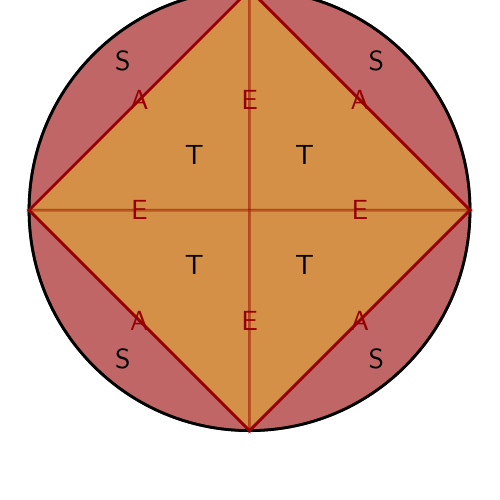
\begin{tikzpicture}[xscale=0.7,yscale=0.7]
 \draw[fill=unirot,opacity=0.6] (4,0) circle [radius=4.0];
 \draw (4,0) circle [radius=4.0];
 \draw[unirot, fill=yellow, opacity=0.3] (0,0) -- (4,4) -- (4,0) -- cycle;
 \draw[unirot, fill=yellow, opacity=0.3] (4,0) -- (4,4) -- (8,0) --cycle;
 \draw[unirot, fill=yellow, opacity=0.3] (0,0) -- (4,-4) -- (4,0) -- cycle;
 \draw[unirot, fill=yellow, opacity=0.3] (4,0) -- (4,-4) -- (8,0) --cycle;
 \draw[unirot] (0,0) -- (4,4) -- (8,0) -- (4,-4) -- cycle;
 \draw (1.7,2.7) node {S};
 \draw (6.3,2.7) node {S};
 \draw (1.7,-2.7) node {S};
 \draw (6.3,-2.7) node {S};
 \draw (3,1) node {T};
 \draw (5,1) node {T};
 \draw (5,-1) node {T};
 \draw (3,-1) node {T};
 \draw[unirot] (4,2) node {E};
 \draw[unirot] (6,0) node {E};
 \draw[unirot] (4,-2) node {E};
 \draw[unirot] (2,0) node {E};
 \draw[unirot] (2,2) node {A};
 \draw[unirot] (6,2) node {A};
 \draw[unirot] (2,-2) node {A};
 \draw[unirot] (6,-2) node {A};
\end{tikzpicture}
\caption{A simple Finite Element grid on the unit square}
\label{fig:fehlersch}
\end{figure}

In  (\ref{fig:fehlersch}), $T$ is an element of the triangulation, $E$ denotes the inner edge between two cells,
$A$ denotes a boundary edge of the discrete space $\Omega_h$ and $S$ a boundary cell between $A$ and $\partial\Omega$ as in Figure \ref{fig:fehlersch}.
That means in particular that the residuals $\rho_{S}$ and $\rho_A$ disappear in the sum over all cells as soon as $T$ is an inner cell, which is not bordering on a boundary cell $S$.
$S_T$ is a boundary cell above an outer cell $T$.
$\rho_E$ is defined over the jump over an inner edge as in Equation \ref{jump}

Clearly, the parts $\rho_T$ describe the classical residual of the Poisson equation $-\Delta u = f$.
The jumps over the edges in $\rho_E$ measure the smoothness of the discrete solution. As a consequence, the edge residuals of $u$
disappear if $u$ is a $C^1$-function, see \cite[page 91]{richterskript}.
For the evaluation of the energy error estimator the data $f$ have to be known and we have to compute the jumps on the respective edges.
Furthermore, we need to compute the outer normal vectors along the boundary edges $A$.
$\rho_S$ must be computed approximatively, as the domain $S_h$ is not known in general.
Especially the constant $c$ as a prefactor of the estimator consists of two constants $c_I$ and $c_T$.
The interpolation constant $c_I$ is usually estimated, too.
The constant $c_T$ which measures the degree of overlapping can be computed; see \cite[page 91]{richterskript}.\\
For the implementation, we cut down on a linear Finite Element ansatz and just solve the Poisson equation on the two dimensional unit circle as the continuous domain.\\

For the proof of the extended error estimator and more details we refer to the source \cite[page 18]{bachelor}.

\subsection{Implementation of the extended a-posteriori error estimator}
To implement the extended error estimator $\| \nabla e_h\|_{L^2(\Omega)} \leq c\ \eta_h$ described in Section \ref{estimator} we need to compute four residual terms.
The cell residuals depend on the discretization parameter $h_T$ and the $L^2$ norm over $\Omega_h$ of the data $f$ or of $f + \Delta u_h$, if we deal with a quadrangular discretization.
For the edge residuals we need to know the length of the edge $h_E$ and the jumps over the current edge.\\
The boundary residuals are defined by the length of the outer edge and the $L^2$- norm on boundary cells $S$ of $f$.
The domain of integration $S$ is usually unknown. However, in case of the unit circle we can approximate $S$ appropriately.
To get $\rho_A$ we require the length of the outer edge and the evaluation of $\nabla u_h$ in the direction of the outer unit normal along the outer edge $A$.\\
Concerning the application of the extended error estimator introduced above for adaptive refinement we propose the following: 
in each step of the refinement we refine on those elements whose local error $\eta_T$ lies above the mean error $\frac{\sum_{T \in \Omega_h}\eta_T}{\#T}$.
Furthermore, we choose an upper bound of $100.000$ cells in order to reduce the run time.\\
To stress the relevance of the additive terms of the new error estimator we will compare in Section \ref{quality} the extended and the standard error estimator.

% Um eine bessere Vergleichbarkeit der Schätzer zu ermöglichen, ist es sinnvoller, dabei so adaptiv zu verfeinern, 
% dass in jedem Schritt ein bestimmter Prozentsatz von Elementen, hier $16\%$,
% verfeinert werden soll.\\
% Allgemein ist diese Verfeinerungsstrategie für das Lösen des ersten einfachen Problems nicht ideal, weil die geschätzten Fehlerwerte sehr dicht beieinander liegen.

\section{The Commented Program}
\subsection{Preliminaries}
HiFlow$^3$ is designed for high performance computing on massively parallel machines. 
So it applies the Message Passing Interface (MPI)\index{Message Passing Interface (MPI)}\index{MPI} library specification for message-passing, see sections \ref{sectionmain}, \ref{read-mesh}, 
\ref{memberComputeError}, \ref{adapt}, \cite{MPI}, \cite{MPIstandard} .\\
The Poisson tutorial needs following two input files:
\begin{itemize}
\item A parameter file: The parameter file is an xml-file, which contains all parameters needed to execute the program. It is read in by the program. 
It is not necessary to recompile the program, when parameters in the xml-file are changed. By default the Poisson adaptive tutorial reads in the parameter file poisson\_adaptive.xml, 
see section \ref{sectionparameter file}, which contains the parameters of a first numerical example, see section \ref{sectionExample}.
This file is stored in \verb'/hiflow/examples/poisson_adaptive/'.  
\item Geometry data\index{geometry data}: The file containing the geometry is specified in the parameter file (poisson\_adaptive.xml). \\
In the numerical example in Section \ref{sectionExample} we used \textbf{unit\_square\_inner\_square.inp}. 
You can find different meshes in the folder \verb'/hiflow/examples/data' .
\end{itemize}

HiFlow$^3$ does not generate meshes\index{mesh!generate} for the domain $\Omega$.\index{domain geometry!generating} Meshes in *.inp and *.vtu format can be read in. 
It is possible to extend the reader for other formats.
Furthermore it is possible to generate other geometries by using external programs (Mesh generators) or by hand.\\  

\subsection{Parameter File}\index{parameter file}\label{sectionparameter file}
The parameters required are initialized in the paramter file poisson\_adaptive.xml.
\begin{lstlisting}[language=XML, basicstyle={\footnotesize, \ttfamily}, keywordstyle=\color{blue}, numbers=none, tabsize=4]
<Param>
    <Mesh>
        <Filename2>L_amr.inp</Filename2>
        <Filename3>unit_cube_amr.inp</Filename3>
        <InitialRefLevel>2</InitialRefLevel>
        <FinalRefLevel>7</FinalRefLevel>
        <FeDegree>1</FeDegree>
        <!-- 1: uniform, 2: adaptive -->
        <Refinement>2</Refinement>
        <!-- 1: cell residuals and jump terms, 2: additional boundary terms -->
        <Estimator>1</Estimator>
        <!-- Refinement strategy: 1: standard: refine all cells with 
            error indicator higher than mean error indicator, 2: refine 
             and coarsen given fraction of cells -->
        <Strategy>1</Strategy>
        <!-- Start coarsening when more than CoarsenThreshold cells 
            are in the mesh -->
        <CoarsenThreshold>400</CoarsenThreshold> 
        <!-- Refine the FractionToRefine * 100% cells with highest
            error indicator -->
        <FractionToRefine>0.2</FractionToRefine>
        <!-- Mark the FractionToRefine * 100% cells with lowest error 
             indicator for coarsening -->
        <FractionToCoarsen>0.2</FractionToCoarsen>
        <!-- Coarsen a family of cells
             if sum_{cell_in_family} (coarsen_flag(cell)) >= 
             #(cells_in_family) -->
        <CoarsenFlag>1</CoarsenFlag> 
        <!-- 2: cells sharing a common vertex differ in one level of
             refinement at most. -->
        <!-- 1: cells sharing a common edge (3D) / vertex (2D) differ in one 
             level of refinement at most. -->
        <!-- 0: cells sharing a common facet differ in one level of refinement 
             at most. -->
        <BalanceConnectionMode>0</BalanceConnectionMode>
        <!-- Sets the level of refinement, starting at which the mesh is 
              always in such a state, that all cells can be coarsened.
              This is realized by refining additional cells -->
        <!-- If set to -1, no patch mode at all -->
        <PatchModeLevel>4</PatchModeLevel>
    </Mesh>
    <LinearAlgebra>
        <NameMatrix>CoupledMatrix</NameMatrix>
        <NameVector>CoupledVector</NameVector>
        <Platform>CPU</Platform>
        <Implementation>Naive</Implementation>
        <MatrixFormat>CSR</MatrixFormat>
    </LinearAlgebra>
    <LinearSolver>
        <Name>CG</Name>
        <SizeBasis>50</SizeBasis>
        <Method>NoPreconditioning</Method>
        <MaxIterations>10000</MaxIterations>
        <AbsTolerance>1.0e-14</AbsTolerance>
        <RelTolerance>1.0e-12</RelTolerance>
        <DivTolerance>1.0e6</DivTolerance>
    </LinearSolver>
</Param>
\end{lstlisting}

\subsection{Structure of the Tutorial}
Following member functions (signed by \textbullet) are defined in the class \texttt{Poisson Adaptive}. The survey reflects the  access relations between the functions, classes and structs. 
 \begin{itemize}
    \item run()
    \item build\_initial\_mesh()
    \item prepare\_system()
    \begin{itemize}
	\item DirichletZero struct (poisson\_adaptive.h)
    \end{itemize}
    \item assemble\_system()
    \begin{itemize}
	\item LocalPoissonAssembler class (poisson\_adaptive.h)
        \begin{itemize}
	    \item ExactSol-struct (poisson\_adaptive.h)
	\end{itemize}    
    \end{itemize}    
    \item solve\_system()
    \item compute\_error()
    \begin{itemize}
	\item L2ErrorIntegrator class (poisson\_adaptive.h)
	\item H1ErrorIntegrator class (poisson\_adaptive.h)    
    \end{itemize}  
    \item error\_estimator()
    \item visualize()
    \item adapt\_uniform()
    \item adapt()
 \end{itemize} 
You can find the source text of every member function in an extra section below. 

\subsection{Main Function}\index{MPI}\label{sectionmain}
The main function starts the simulation of the Poisson problem (poisson\_adaptive.cc).

\begin{lstlisting}[language=C++, basicstyle={\footnotesize, \ttfamily}, keywordstyle=\color{blue}, numbers=none, tabsize=4]
// Program entry point
int main ( int argc, char** argv )
{
    MPI_Init ( &argc, &argv );

    // Set default parameter file
    std::string param_filename ( PARAM_FILENAME );
    std::string path_mesh;
    // If set take parameter file specified on console
    if ( argc > 1 )
    {
        param_filename = std::string ( argv[1] );
    }
    // If set take mesh following path specified on console
    if ( argc > 2 )
    {
        path_mesh = std::string ( argv[2] );
    }
    try
    {
        // Create log files for INFO and DEBUG output
        //    std::ofstream info_log("poisson_tutorial_info_log");
        LogKeeper::get_log ( "info" ).set_target ( &( std::cout ) );
        //std::ofstream debug_log("poisson_tutorial_debug_log");
        LogKeeper::get_log ( "debug" ).set_target ( &( std::cout ) );
        //     std::ofstream error_log ( "poisson_tutorial_error_log" );
        LogKeeper::get_log ( "error" ).set_target ( &( std::cout ) );

        // Create application object and run it
        PoissonAdaptive app ( param_filename, path_mesh );

        app.run ( );

    }
    catch ( std::exception& e )
    {
        std::cerr << "\nProgram ended with uncaught exception.\n";
        std::cerr << e.what ( ) << "\n";
        return -1;
    }
    MPI_Finalize ( );
    return 0;
}
\end{lstlisting}

\subsection{Member Functions}
\subsubsection{run()}
The member function run() is defined in the class \texttt{Poisson Adaptive} (poisson\_adaptive.cc).

\begin{lstlisting}[language=C++, basicstyle={\footnotesize, \ttfamily}, keywordstyle=\color{blue}, numbers=none, tabsize=4]
    void run ( )
    {
        int patch_mode_level = params_["Mesh"]["PatchModeLevel"].
             get<int>( -1 );

        // Prepare headers of CSV file
        this->csv_names_.clear ( );
        this->csv_names_.push_back ( "Level" );
        this->csv_names_.push_back ( "Global number of DoFs " );
        this->csv_names_.push_back ( "Setup system time " );
        this->csv_names_.push_back ( "Assembly time " );
        this->csv_names_.push_back ( "Solve time " );
        this->csv_names_.push_back ( "Compute Error time " );
        this->csv_names_.push_back ( "L2 error " );
        this->csv_names_.push_back ( "H1 error " );
        this->csv_names_.push_back ( "Error estimator time " );
        this->csv_names_.push_back ( "Std estimator " );
        this->csv_names_.push_back ( "Patch interpolation time " );
        this->csv_names_.push_back ( "Mesh Adapt time " );
        this->csv_names_.push_back ( "Mesh Ghost time " );

        if ( this->rank_ == MASTER_RANK )
        {
            std::stringstream csv_file_name;
            csv_file_name << this->num_partitions_ << "_statistics.csv";
            this->csv_writer_.InitFilename ( csv_file_name.str ( ) );
            this->csv_writer_.Init ( this->csv_names_ );
        }

        // Construct / read in the initial mesh.
        build_initial_mesh ( );

        // Main adaptation loop.
        while ( !is_done_ )
        {
            // Prepare data for statistics in CSV file
            this->csv_quantities_.clear ( );

            // Add current refinement level
            this->csv_quantities_.push_back ( this->refinement_level_ );

            LOG_INFO ( "Refinement Level", " ===== " << refinement_level_ << 
                       "\n=====" );

            // Initialize space and linear algebra.
            prepare_system ( );

            // Compute the stiffness matrix and right-hand side.
            assemble_system ( );

            // Solve the linear system.
            solve_system ( );

            // Compute the error to the exact solution.
            // Includes the A posteriori error estimator.
            compute_error ( );
            error_estimator ( );

            // Visualize the solution and the errors.
            visualize ( );

#ifdef USE_MESH_P4EST
            // higher order patch interpolation
            if ( refinement_level_ > patch_mode_level && 
                 patch_mode_level >= 0 )
            {
                LOG_INFO ( "Higher order interpolation", true );
                higher_order_interpolation ( );
            }
            else
            {
                this->csv_quantities_.push_back ( 0.0 );
            }
#endif
            LOG_INFO ( "Visualize", true );
            // Uniform or adaptive refinement
            int refinement_ = params_["Mesh"]["Refinement"].get<int>( 3 );
            if ( refinement_ == 1 )
            {
                adapt_uniform ( );
                LOG_INFO ( "Adapt uniform", true );
            }
            else
            {
                adapt ( );
                LOG_INFO ( "Adapt locally", true );
                LOG_INFO ( "Is done", is_done_ );
            }

            // Write CSV output
            if ( this->rank_ == MASTER_RANK )
            {
                this->csv_writer_.write ( this->csv_quantities_ );
            }
        }
    }
\end{lstlisting}

\subsubsection{build\_initial\_mesh()}\index{MPI}\label{read-mesh}
This member function, defined in the class \texttt{Poisson Adaptive}, reads the initial mesh (poisson\_adaptive.cc), and writes out the refined mesh of initial refinement level.

\begin{lstlisting}[language=C++, basicstyle={\footnotesize, \ttfamily}, keywordstyle=\color{blue}, numbers=none, tabsize=4]
void PoissonAdaptive::build_initial_mesh ( )
{
    Timer timer;
    timer.start ( );

    // Read in the mesh.
    //The mesh is chosen according to the dimension of the problem.
    std::string mesh_name;

    if ( DIMENSION == 2 )
    {
        mesh_name = params_["Mesh"]["Filename2"].get<std::string>
             ( "unit_square_inner_square.inp" );
#ifdef ELLIPSOID_BOUNDARY
        mesh_name = "unit_square_inner_square.inp";
#endif
    }
    if ( DIMENSION == 3 )
    {
        mesh_name = params_["Mesh"]["Filename3"].
            get<std::string>( "unit_cube.inp" );
    }

    std::string mesh_filename;
    if ( path_mesh.empty ( ) )
    {
        mesh_filename = std::string ( DATADIR ) + mesh_name;
    }
    else
    {
        mesh_filename = path_mesh + mesh_name;
    }

    std::vector<MasterSlave> period ( 0, MasterSlave ( 0., 0., 0., 0 ) );

    SharedVertexTable shared_verts;
    if ( rank_ == MASTER_RANK )
    {
#ifdef USE_MESH_P4EST
        master_mesh_ = read_mesh_from_file ( mesh_filename, DIMENSION, DIMENSION, 
                                             0, period, mesh::IMPL_P4EST );
#else
        master_mesh_ = read_mesh_from_file ( mesh_filename, DIMENSION, DIMENSION, 
                                             0, period, mesh::IMPL_DBVIEW );
#endif
        // Refine the mesh until the initial refinement level is reached.
        const int initial_ref_lvl = params_["Mesh"]["InitialRefLevel"].
            get<int>( 3 );
        if ( initial_ref_lvl > 0 )
        {
            LOG_DEBUG ( 1, "Initial refinement level " << initial_ref_lvl );
            master_mesh_ = master_mesh_->refine_uniform_seq ( initial_ref_lvl );
            //master_mesh_->do_tests(0);
        }
        refinement_level_ = initial_ref_lvl;
    }
    // Broadcast information from master to slaves.
    MPI_Bcast ( &refinement_level_, 1, MPI_INT, MASTER_RANK, comm_ );
    int uniform_ref_steps;

#ifdef USE_MESH_P4EST
    mesh_ = partition_and_distribute ( master_mesh_, MASTER_RANK, comm_, 
                                       &uniform_ref_steps, mesh::IMPL_P4EST );
    mesh_ = compute_ghost_cells ( *mesh_, comm_, shared_verts, mesh::IMPL_P4EST, 2 );
    if ( rank_ == 0 )
    {
        //mesh_->do_tests(1);
    }
#else
    mesh_without_ghost_ = partition_and_distribute ( master_mesh_, MASTER_RANK, 
                                                     comm_, 
                                                     &uniform_ref_steps, 
                                                     mesh::IMPL_DBVIEW );
    mesh_ = compute_ghost_cells ( *mesh_without_ghost_, comm_, shared_verts, 
                                  mesh::IMPL_DBVIEW, 1 );
#endif

    refinement_level_ += uniform_ref_steps;
    // Add subdomain and remote index information needed by the library
    if ( num_partitions_ == 1 )
    {
        std::vector<int> remote_index
                (
                  mesh_->num_entities ( mesh_->tdim ( ) ),
                  -1
                  );

        AttributePtr remote_index_attr ( new IntAttribute ( remote_index ) );
        mesh_->add_attribute ( "_remote_index_",
                               DIMENSION,
                               remote_index_attr );

        std::vector<int> subdomain
                ( mesh_->num_entities ( mesh_->tdim ( ) ),
                  0
                  );
        AttributePtr subdomain_attr ( new IntAttribute ( subdomain ) );
        mesh_->add_attribute ( "_sub_domain_",
                               DIMENSION,
                               subdomain_attr );
    }

#ifdef ELLIPSOID_BOUNDARY
    // circle with radius = 1
    Coordinate radius = 1.;
    Ellipsoid circle ( radius, radius );
    adapt_boundary_to_function ( mesh_, circle );

    // Refine the mesh until the initial refinement level is reached.
    const int initial_ref_lvl = params_["Mesh"]["InitialRefLevel"].
        get<int>( 3 );

    for ( int r = 0; r < initial_ref_lvl; ++r )
    {
        adapt_boundary_to_function ( mesh_, circle );
        ++refinement_level_;
    }
#endif

    timer.stop ( );
    LOG_INFO ( "Build initial mesh time ", timer.get_duration ( ) );
    this->csv_quantities_.push_back ( timer.get_duration ( ) );

    PVtkWriter writer ( comm_ );
    std::ostringstream name;
    name << "poisson_adaptive_initial_mesh.pvtu";
    std::string output_file = name.str ( );
    writer.add_all_attributes ( *mesh_, true );
    writer.write ( output_file.c_str ( ), *mesh_ );
}
\end{lstlisting}
\subsubsection{prepare\_system()}
The member function prepare\_system() initializes the space and the linear algebra (poisson\_adaptive.cc). 
The polynomial degree of the Finite Element functions is set to the parameter "FeDegree" defined in the parameter file. 
The size and the non-zero pattern of the stiffness matrix matrix\_ is initialized. 
The vectors for the right-hand side rhs\_, and the solution are initialized and set to a zero vector of the correct size.

\begin{lstlisting}[language=C++, basicstyle={\footnotesize, \ttfamily}, keywordstyle=\color{blue}, numbers=none, tabsize=4]
void PoissonAdaptive::prepare_system ( )
{
    Timer timer;
    timer.start ( );

#ifndef WITH_HYPRE
    if ( matrix_ != NULL )
    {
        delete matrix_;
    }
    if ( rhs_ != NULL )
    {
        delete rhs_;
    }
    if ( sol_ != NULL )
    {
        delete sol_;
    }
    if ( exact_sol_ != NULL )
    {
        delete exact_sol_;
    }

    matrix_ = new CoupledMatrix<Scalar>;
    rhs_ = new CoupledVector<Scalar>;
    sol_ = new CoupledVector<Scalar>;
    exact_sol_ = new CoupledVector<Scalar>;
#endif

    // Assign degrees to each element.
    const int fe_degree = params_["Mesh"]["FeDegree"].get<int>( 1 );
    std::vector< int > degrees ( 1, fe_degree );

    // Initialize the VectorSpace object.
    space_.Clear ( );
    space_.Init ( degrees, *mesh_ );

    this->csv_quantities_.push_back ( space_.dof ( ).ndofs_global ( ) );

    // Setup couplings object.
    couplings_.Clear ( );
    couplings_.Init ( comm_, space_.dof ( ) );

    // Compute the matrix graph.
    SparsityStructure sparsity;
    global_asm_.compute_sparsity_structure ( space_, sparsity );

    couplings_.InitializeCouplings ( sparsity.off_diagonal_rows,
                                     sparsity.off_diagonal_cols );

#ifdef WITH_HYPRE
    matrix_.Init ( comm_, couplings_ );
    matrix_.InitStructure ( vec2ptr ( sparsity.diagonal_rows ),
                            vec2ptr ( sparsity.diagonal_cols ),
                            sparsity.diagonal_rows.size ( ),
                            vec2ptr ( sparsity.off_diagonal_rows ),
                            vec2ptr ( sparsity.off_diagonal_cols ),
                            sparsity.off_diagonal_rows.size ( ) );
    //matrix_hypre_.print_statistics();

    rhs_.Init ( comm_, couplings_ );
    sol_.Init ( comm_, couplings_ );
    exact_sol_.Init ( comm_, couplings_ );
    //rhs_hypre_.print_statistics();
    //sol_hypre_.print_statistics();
#else

    matrix_->Init ( comm_, couplings_, CPU, NAIVE, CSR );
    rhs_->Init ( comm_, couplings_, CPU, NAIVE );
    sol_->Init ( comm_, couplings_, CPU, NAIVE );
    exact_sol_->Init ( comm_, couplings_, CPU, NAIVE );

    // Initialize structure of LA objects.
    matrix_->InitStructure ( vec2ptr ( sparsity.diagonal_rows ),
                             vec2ptr ( sparsity.diagonal_cols ),
                             sparsity.diagonal_rows.size ( ),
                             vec2ptr ( sparsity.off_diagonal_rows ),
                             vec2ptr ( sparsity.off_diagonal_cols ),
                             sparsity.off_diagonal_rows.size ( ) );

    rhs_->InitStructure ( );
    sol_->InitStructure ( );
    exact_sol_->InitStructure ( );

    // Zero all linear algebra objects.
    matrix_->Zeros ( );
    rhs_->Zeros ( );
    sol_->Zeros ( );
    exact_sol_->Zeros ( );
#endif

    // Compute Dirichlet BC dofs and values using known exact solution.
    dirichlet_dofs_.clear ( );
    dirichlet_values_.clear ( );

    DirichletZero zero;

    // The function compute_dirichlet_dofs_and_values des not yet work 
    // for 1D.
    if ( DIMENSION == 1 )
    {
        dirichlet_values_.resize ( 2, 0.0 );

        // Loop over all cells.
        for ( EntityIterator facet_it = mesh_->begin ( DIMENSION - 1 ),
              facet_end = mesh_->end ( DIMENSION - 1 );
              facet_it != facet_end;
              ++facet_it )
        {

            // Returns the number of neighbors for each cell to check
            // if it is on the facet.
            const EntityCount num_cell_neighbors = facet_it
                    ->num_incident_entities
                    ( DIMENSION );

            // If it lies on the facet, the corresponding DOF is a Dirichlet
            // DOF and is added to dirichlet_dofs_.
            if ( num_cell_neighbors == 1 )
            {
                std::vector<int> dof_number_;
                space_.dof ( ).get_dofs_on_subentity
                        (
                          0,
                          facet_it->begin_incident ( DIMENSION )->index ( ),
                          0,
                          facet_it->index ( ),
                          dof_number_
                          );
                dirichlet_dofs_.push_back ( dof_number_[0] );
            }
        }
    }
        //homogeneous Dirichlet boundaries
    else
    {
        compute_dirichlet_dofs_and_values ( zero, space_, 0, dirichlet_dofs_,
                                            dirichlet_values_ );
    }
    timer.stop ( );
    LOG_INFO ( "Space setup time ", timer.get_duration ( ) );
    this->csv_quantities_.push_back ( timer.get_duration ( ) );
}
\end{lstlisting}

\textbf{struct DirichletZero} \label{structDirichletZero}\index{boundary condition!modelling}\\
This struct in poisson\_adaptive.h defines the homogeneous Dirichlet boundary condition, given in (\ref{poisson_equation}).
\begin{lstlisting}[language=C++, basicstyle={\footnotesize, \ttfamily}, keywordstyle=\color{blue}, numbers=none, tabsize=4]
// Dirichlet boundary condition
// Functor used to impose u = 0 on the boundary.
struct DirichletZero
{

    std::vector<double> evaluate (
                                   const mesh::Entity& face,
                                   const std::vector<Coord>& coords_on_face
                                   ) const
    {
        // return array with Dirichlet values for dof:s on boundary face
        if ( face.get_material_number ( ) == 11 )
        {
            return std::vector<double>( coords_on_face.size ( ), 0.0 );
        }
        // Neumann boundary values
        return std::vector<double>( 0, 0.0 );
    }
};
\end{lstlisting}

\subsubsection{assemble\_system()}
The member function assemble\_system() computes the stiffness matrix\index{stiffness matrix!assembling} and right-hand side\index{right-hand side!assembling} (poisson\_adaptive.cc). The stiffness matrix, right-hand side vector and solution vector are modified to set correct Dirichlet values for the boundary DoFs.

\begin{lstlisting}[language=C++, basicstyle={\footnotesize, \ttfamily}, keywordstyle=\color{blue}, numbers=none, tabsize=4]
void PoissonAdaptive::assemble_system ( )
{
    Timer assembly_hf_la;
    assembly_hf_la.start ( );

    // Assemble matrix and right-hand-side vector.
    LocalPoissonAssembler<ExactSol> local_asm;
#ifdef WITH_HYPRE
    global_asm_.assemble_matrix ( space_, local_asm, matrix_ );
    global_asm_.assemble_vector ( space_, local_asm, rhs_ );
#else
    global_asm_.assemble_matrix ( space_, local_asm, *matrix_ );
    global_asm_.assemble_vector ( space_, local_asm, *rhs_ );
#endif

    assembly_hf_la.stop ( );
    LOG_INFO ( "Assembly time with HiFlow LA", 
               assembly_hf_la.get_duration ( ) );
    this->csv_quantities_.push_back ( assembly_hf_la.get_duration ( ) );

#ifdef WITH_HYPRE
    if ( !dirichlet_dofs_.empty ( ) )
    {
        // Correct Dirichlet dofs.
        matrix_.diagonalize_rows ( vec2ptr ( dirichlet_dofs_ ),
                                   dirichlet_dofs_.size ( ), 1.0 );
        rhs_.SetValues ( vec2ptr ( dirichlet_dofs_ ), dirichlet_dofs_.size ( ),
                         vec2ptr ( dirichlet_values_ ) );
        sol_.SetValues ( vec2ptr ( dirichlet_dofs_ ), dirichlet_dofs_.size ( ),
                         vec2ptr ( dirichlet_values_ ) );
    }
    sol_.Update ( );
    rhs_.Update ( );
#else
    if ( !dirichlet_dofs_.empty ( ) )
    {
        // Correct Dirichlet dofs.
        matrix_->diagonalize_rows ( vec2ptr ( dirichlet_dofs_ ),
                                    dirichlet_dofs_.size ( ), 1.0 );
        rhs_->SetValues ( vec2ptr ( dirichlet_dofs_ ), dirichlet_dofs_.size ( ),
                          vec2ptr ( dirichlet_values_ ) );
        sol_->SetValues ( vec2ptr ( dirichlet_dofs_ ), dirichlet_dofs_.size ( ),
                          vec2ptr ( dirichlet_values_ ) );
    }
    sol_->UpdateCouplings ( );
    rhs_->UpdateCouplings ( );
#endif

    ExactSol exact_sol_fn;
    for ( mesh::EntityIterator it = mesh_->begin ( DIMENSION ), 
          end_it = mesh_->end ( DIMENSION ); it != end_it; ++it )
    {
        std::vector<int> global_dof_ids;
        space_.GetDofIndices ( 0, *it, &global_dof_ids );
        int num_dofs = global_dof_ids.size ( );
        std::vector<double> values;
        values.resize ( num_dofs, 0. );

        std::vector< Coord > coords;
        space_.dof ( ).get_coord_on_cell ( 0, it->index ( ), coords );
        for ( int i = 0; i < num_dofs; i++ )
        {
            if ( rank_ == space_.dof ( ).owner_of_dof ( global_dof_ids.at ( i ) ) )
            {
                Vec<DIMENSION, double> pt;
                for ( int l = 0; l < DIMENSION; ++l )
                {
                    pt[l] = coords[i][l];
                }
                double val = exact_sol_fn ( pt );
#ifdef WITH_HYPRE
                exact_sol_.SetValues ( &global_dof_ids.at ( i ), 1, &val );
#else
                exact_sol_->SetValues ( &global_dof_ids.at ( i ), 1, &val );
#endif
            }

            if ( DEBUG_LEVEL >= 3 )
            {
                if ( rank_ == space_.dof ( ).owner_of_dof ( global_dof_ids.at ( i ) ) )
                {
                    double val;
#ifdef WITH_HYPRE
                    matrix_.GetValues ( &global_dof_ids.at ( i ), 1, 
                                        &global_dof_ids.at ( i ), 1, &val );
#else
                    matrix_->GetValues ( &global_dof_ids.at ( i ), 1, 
                                         &global_dof_ids.at ( i ), 1, &val );
#endif

                    if ( val == 1. )
                    {
                        LOG_DEBUG ( 3, "[" << rank_ << "] Dof id " << 
                                    global_dof_ids.at ( i ) << 
                                    " has diagonal entry " << val << " and coord " 
                                    << coords[i][0] << ", " << coords[i][1] );
                    }
                }
            }
        }
    }

#ifdef WITH_HYPRE
    exact_sol_.Update ( );
    interpolate_constrained_vector ( space_, exact_sol_ );
    exact_sol_.Update ( );
#else
    exact_sol_->UpdateCouplings ( );
    interpolate_constrained_vector ( space_, *exact_sol_ );
    exact_sol_->UpdateCouplings ( );
#endif
}
\end{lstlisting} 

\textbf{LocalPoissonAssembler class}\\
This class implements the stiffness matrix and right-hand side locally for each cell.

\begin{lstlisting}[language=C++, basicstyle={\footnotesize, \ttfamily}, keywordstyle=\color{blue}, numbers=none, tabsize=4]
// Assembling of the linear system
// Functor used for the local assembly of the stiffness matrix and load vector.
template<class ExactSol>
class LocalPoissonAssembler : private AssemblyAssistant<DIMENSION, double>
{
  public:

    void operator() ( const Element<double>& element,
            const Quadrature<double>& quadrature,
            LocalMatrix& lm )
    {
        AssemblyAssistant<DIMENSION, double>::initialize_for_element
                ( element, quadrature );

        // Local stiffness matrix
        const int num_q = num_quadrature_points ( );
        for ( int q = 0; q < num_q; ++q )
        {
            const double wq = w ( q );
            const int n_dofs = num_dofs ( 0 );
            for ( int i = 0; i < n_dofs; ++i )
            {
                for ( int j = 0; j < n_dofs; ++j )
                {
                    lm ( dof_index ( i, 0 ), dof_index ( j, 0 ) ) +=
                            wq
                            * dot ( grad_phi ( j, q ), grad_phi ( i, q ) )
                            * std::abs ( detJ ( q ) );
                }
            }
        }
    }

    void operator() ( const Element<double>& element,
            const Quadrature<double>& quadrature,
            LocalVector& lv )
    {
        AssemblyAssistant<DIMENSION, double>::initialize_for_element
                ( element, quadrature );

        const int num_q = num_quadrature_points ( );
        for ( int q = 0; q < num_q; ++q )
        {
            const double wq = w ( q );
            const int n_dofs = num_dofs ( 0 );
            for ( int i = 0; i < n_dofs; ++i )
            {
                lv[dof_index ( i, 0 )] += wq
                        * f ( x ( q ) ) * phi ( i, q )
                        * std::abs ( detJ ( q ) );
            }
        }
    }

};
 // Right hand side f

double f ( Vec<DIMENSION, double> pt )
{
    ExactSol sol;
    double rhs_sol;
#ifdef ELLIPSOID_BOUNDARY
    const double x = pt[0];
    const double y = ( DIMENSION > 1 ) ? pt[1] : 0;
    const double pi = M_PI;
    const double a = 1.;
    const double b = 1.;
    const double k = 10.0;
    rhs_sol = 8.
            * k
            * std::pow ( ( x * x ) / ( a * a )+( y * y ) / ( b * b ), 4. * k )
            * (
            a * a * a * a * ( 8. * k - 1 ) * y * y
            + a * a * b * b * ( x * x + y * y )
            + b * b * b * b * ( 8. * k - 1 ) * x * x
            )
            / (
            std::pow ( a * a * y * y + b * b * x*x, 2 )
            );
#else
#    ifdef CONST_F
    rhs_sol = 1;
#    else
    switch ( DIMENSION )
    {
        case 1:
        {
            rhs_sol = 4. * M_PI * M_PI * ( M * M ) * sol ( pt );
            break;
        }
        case 2:
        {
            rhs_sol = 4. * M_PI * M_PI * ( M * M + N * N ) * sol ( pt );
            break;
        }
        case 3:
        {
            rhs_sol = 4. * M_PI * M_PI * ( M * M + N * N + O * O ) * sol ( pt );
            break;
        }
    }
#    endif
#endif
    return rhs_sol;
}
\end{lstlisting}

\textbf{ExactSol struct}\label{structExactSol}\\
The struct ExactSol in poisson\_adaptive.h implements the exact solution \index{solution!exact} $u$ given by (\ref{exactSolution}) and the exact gradient $\nabla u$.

\begin{lstlisting}[language=C++, basicstyle={\footnotesize, \ttfamily}, keywordstyle=\color{blue}, numbers=none, tabsize=4]
// Exact solution
struct ExactSol
{

    double operator() ( const Vec<DIMENSION, double>& pt ) const
    {
        const double x = pt[0];
        const double y = ( DIMENSION > 1 ) ? pt[1] : 0;
        const double z = ( DIMENSION > 2 ) ? pt[2] : 0;
        double solution;
#ifdef ELLIPSOID_BOUNDARY
        // a and b are the axes of the ellipse geometry
        // unit circle a = b = 1
        const double a = 1.;
        const double b = 1.;
        const double k = 10.0;
        solution = -std::pow ( ( ( x / a )*( x / a )+( y / b )*( y / b ) ),
                               4. * k )
                + 1.;
#else
        const double pi = M_PI;
        switch ( DIMENSION )
        {
            case 1:
            {
                solution = 10.0 * std::sin ( 2. * M * pi * x );
                break;
            }
            case 2:
            {
                solution = 10.0 * std::sin ( 2. * M * pi * x ) * 
                                  std::sin ( 2. * N * pi * y );
                break;
            }
            case 3:
            {
                solution = 10.0 * std::sin ( 2. * M * pi * x ) * 
                                  std::sin ( 2. * N * pi * y ) * 
                                  std::sin ( 2. * O * pi * z );
                break;
            }
        }
#endif
        return solution;
    }

    // Partial derivations of the exact solution

    Vec<DIMENSION, double> eval_grad ( const Vec<DIMENSION, double>& pt ) const
    {
        Vec<DIMENSION, double> grad;
        const double x = pt[0];
        const double y = ( DIMENSION > 1 ) ? pt[1] : 0;

#ifdef ELLIPSOID_BOUNDARY
        const double a = 1.;
        const double b = 1.;
        const double k = 10.0;
        grad[0] = -4. * k * std::pow ( ( x / a )*( x / a )+( y / b )*( y / b ),
                                       ( 4. * k - 1. ) )
                * ( 2. / ( a * a ) )
                * x;

        grad[1] = -4. * k * std::pow ( ( x / a )*( x / a )+( y / b )*( y / b ),
                                       ( 4. * k - 1. ) )
                * ( 2. / ( b * b ) )
                * y;
#else
        const double z = ( DIMENSION > 2 ) ? pt[2] : 0;
        const double pi = M_PI;

        switch ( DIMENSION )
        {
            case 1:
            {
                grad[0] = 20. * M * pi * std::cos ( 2. * M * pi * x );
                break;
            }
            case 2:
            {
                grad[0] = 20. * M * pi * std::cos ( 2. * M * pi * x ) *
                        std::sin ( 2. * N * pi * y );
                grad[1] = 20. * N * pi * std::sin ( 2. * M * pi * x ) *
                        std::cos ( 2. * N * pi * y );
                break;
            }
            case 3:
            {
                grad[0] = 20. * M * pi * std::cos ( 2. * M * pi * x ) *
                        std::sin ( 2. * N * pi * y ) * 
                        std::sin ( 2. * O * pi * z );
                grad[1] = 20. * N * pi * std::sin ( 2. * M * pi * x ) *
                        std::cos ( 2. * N * pi * y ) * 
                        std::sin ( 2. * O * pi * z );
                grad[2] = 20. * O * pi * std::sin ( 2. * M * pi * x ) *
                        std::sin ( 2. * N * pi * y ) * 
                        std::cos ( 2. * O * pi * z );
                break;
            }
        }
#endif
        return grad;
    }
};

\end{lstlisting}
\subsubsection{solve\_system()}
The member function solve\_system() solves \index{solver} the linear system (poisson\_adaptive.cc). 
The solver is specified in the parameter file. 
The Poisson equation is symmetric positive definite, which means that the CG-method is a good choice, see \ref{sectionparameter file}.

\begin{lstlisting}[language=C++, basicstyle={\footnotesize, \ttfamily}, keywordstyle=\color{blue}, numbers=none, tabsize=4]
void PoissonAdaptive::solve_system ( )
{
    Timer timer;
    timer.start ( );

    const int max_iter = params_["LinearSolver"]["MaxIterations"].
        get<int>( 1000 );
    const double abs_tol = params_["LinearSolver"]["AbsTolerance"].
        get<double>( 1e-12 );
    const double rel_tol = params_["LinearSolver"]["RelTolerance"].
        get<double>( 1e-6 );
    const double div_tol = params_["LinearSolver"]["DivTolerance"].
        get<double>( 1e6 );
    const int basis_size = params_["LinearSolver"]["SizeBasis"].
        get<int>( 100 );
    const std::string solver_type = params_["LinearSolver"]["Name"].
        get<std::string>( "GMRES" );
    const std::string method = params_["LinearSolver"]["Method"].
        get<std::string>( "NoPreconditioning" );

#ifdef WITH_HYPRE
    HypreCG<LAD> solver_hypre;

    solver_hypre.SetupOperator ( matrix_ );
    solver_hypre.InitControl ( max_iter, abs_tol, rel_tol );
    solver_hypre.SetPrintLevel ( 0 );

    HypreBoomerAMG<LAD> precond_boomer;
    precond_boomer.InitControl ( 1, 0., 0. );
    precond_boomer.SetCycleType ( 2 );
    precond_boomer.SetRelaxType ( 6 );
    //precond_boomer.SetCycleRelaxType ( 6, 3 );
    precond_boomer.SetCycleNumSweeps ( 3, 1 );
    precond_boomer.SetCycleNumSweeps ( 3, 2 );
    precond_boomer.SetRelaxWt ( 0.5 );
    precond_boomer.SetCoarsenType ( 10 );
    precond_boomer.SetInterpType ( 6 );
#    if DIMENSION == 2
    precond_boomer.SetStrongThreshold ( 0.25 );
#    else
    precond_boomer.SetStrongThreshold ( 0.6 );
#    endif
    precond_boomer.SetAggNumLevels ( 25 );
    precond_boomer.SetSmoothType ( 0 );
    precond_boomer.SetupOperator ( matrix_ );

    precond_boomer.SetPrintLevel ( 0 );

    precond_boomer.Build ( );

    solver_hypre.SetupPreconditioner ( precond_boomer );

    solver_hypre.Solve ( rhs_, &sol_ );
#else
    LinearSolver<LAD>* solver;
    GMRES<LAD> solver_gmres;
    CG<LAD> solver_cg;

    if ( solver_type == "GMRES" )
    {
        solver = &solver_gmres;
        solver_gmres.InitParameter ( basis_size, method );
    }
    else if ( solver_type == "CG" )
    {
        solver = &solver_cg;
    }
    else
    {
        std::cout << " Solver Type not supported! Exit now " << std::endl;
        exit ( -1 );
    }

    solver->InitControl ( max_iter, abs_tol, rel_tol, div_tol );
    solver->SetPrintLevel ( 0 );

    PreconditionerBlockJacobiStand<LAD> precond;
    precond.InitParameter ( );
    precond.Init_SSOR ( 1.3 );

    precond.SetupOperator ( *matrix_ );
    if ( method != "NoPreconditioning" )
    {
        solver->SetupPreconditioner ( precond );
    }

    solver->SetupOperator ( *matrix_ );
    solver->Solve ( *rhs_, sol_ );
#endif

#ifdef WITH_HYPRE
    sol_.Update ( );
    interpolate_constrained_vector ( space_, sol_ );
    sol_.Update ( );
#else
    sol_->UpdateCouplings ( );
    interpolate_constrained_vector ( space_, *sol_ );
    sol_->UpdateCouplings ( );
#endif

    timer.stop ( );
#ifdef WITH_HYPRE
    LOG_INFO ( "Linear solver", " iter " << solver_hypre.iter ( ) << 
               " CG res " << solver_hypre.res ( ) );
#else
    LOG_INFO ( "Linear solver", " iter " << solver->iter ( ) << 
               " CG res " << solver->res ( ) );
#endif
    LOG_INFO ( "Solving time ", timer.get_duration ( ) );
    this->csv_quantities_.push_back ( timer.get_duration ( ) );

}
\end{lstlisting}

\subsubsection{compute\_error()}\label{memberComputeError}\index{error!computation}\index{MPI}
This member function in poisson\_adaptive.cc computes the error between the approximated and the exact solution mentioned in Section \ref{sectionExample} in the $L^2$ norm and $H^1$ seminorm.

\begin{lstlisting}[language=C++, basicstyle={\footnotesize, \ttfamily}, keywordstyle=\color{blue}, numbers=none, tabsize=4]
void PoissonAdaptive::compute_error ( )
{
    Timer timer;
    timer.start ( );

    // Compute square of the L2 error on each element, putting the
    // values into L2_err_.
    L2_err_.clear ( );
#ifdef WITH_HYPRE
    L2ErrorIntegrator<ExactSol> L2_int ( sol_ );
#else
    L2ErrorIntegrator<ExactSol> L2_int ( *( sol_ ) );
#endif
    global_asm_.assemble_scalar ( space_, L2_int, L2_err_ );

    // Create attribute with L2 error for output.
    AttributePtr L2_err_attr ( new DoubleAttribute ( L2_err_ ) );

    mesh_->add_attribute ( "L2 error", DIMENSION, L2_err_attr );
    double total_L2_err = std::accumulate
            (
              L2_err_.begin ( ),
              L2_err_.end ( ),
              0.
              );
    double global_L2_err = 0.;
    MPI_Allreduce ( &total_L2_err,
                    &global_L2_err,
                    1,
                    MPI_DOUBLE,
                    MPI_SUM,
                    comm_ );
    LOG_INFO ( "error", "Local L2 error on partition " << rank_ << " = " 
               << std::sqrt ( total_L2_err ) );

    // Compute square of the H1 error on each element, putting the
    // values into H1_err_.
    H1_err_.clear ( );
#ifdef WITH_HYPRE
    H1ErrorIntegrator<ExactSol> H1_int ( sol_ );
#else
    H1ErrorIntegrator<ExactSol> H1_int ( *( sol_ ) );
#endif
    global_asm_.assemble_scalar ( space_, H1_int, H1_err_ );

    AttributePtr H1_err_attr ( new DoubleAttribute ( H1_err_ ) );
    mesh_->add_attribute ( "H1 error", DIMENSION, H1_err_attr );
    double total_H1_err = std::accumulate
            (
              H1_err_.begin ( ),
              H1_err_.end ( ),
              0.
              );
    double global_H1_err = 0.;
    MPI_Allreduce ( &total_H1_err,
                    &global_H1_err,
                    1,
                    MPI_DOUBLE,
                    MPI_SUM,
                    comm_ );
    timer.stop ( );
    this->csv_quantities_.push_back ( timer.get_duration ( ) );
    this->csv_quantities_.push_back ( std::sqrt ( global_L2_err ) );
    this->csv_quantities_.push_back ( std::sqrt ( global_H1_err ) );

    LOG_INFO ( "error", "Local H1 error on partition " << rank_ << " = " 
               << std::sqrt ( total_H1_err ) );

    // Output on consol: number of elements and global H^1 error
    if ( rank_ == MASTER_RANK )
    {
        LOG_INFO ( "error", "H1size: " << L2_err_.size ( ) << ", H1 error: "
                   << std::sqrt ( global_H1_err ) );
    }
}
\end{lstlisting}

\textbf{L2ErrorIntegrator class}\\
The class L2ErrorIntegrator implements the evaluation of the square of the $L^2$ norm of the error on each element (poisson\_adaptive.h).

\begin{lstlisting}[language=C++, basicstyle={\footnotesize, \ttfamily}, keywordstyle=\color{blue}, numbers=none, tabsize=4]
// Functor used for the local evaluation of the square of the L2-norm of the
// error on each element.
template<class ExactSol>
class L2ErrorIntegrator : private AssemblyAssistant<DIMENSION, double>
{
  public:

    L2ErrorIntegrator ( CVector& pp_sol )
    : pp_sol_ ( pp_sol )
    {
    }

    void operator() ( const Element<double>& element,
            const Quadrature<double>& quadrature,
            double& value )
    {
        AssemblyAssistant<DIMENSION, double>::initialize_for_element
                ( element, quadrature );

        // Evaluate the computed solution at all quadrature points.
        approx_sol_.clear ( );
        evaluate_fe_function ( pp_sol_, 0., approx_sol_ );

        const int num_q = num_quadrature_points ( );
        for ( int q = 0; q < num_q; ++q )
        {
            const double wq = w ( q );
            // Delta is the quadrature point wise error.
            const double delta = sol_ ( x ( q ) ) - approx_sol_[q];
            value += wq * delta * delta * std::abs ( detJ ( q ) );
        }
    }

  private:
    // Coefficients of the computed solution
    const CVector& pp_sol_;
    // functor to evaluate exact solution
    ExactSol sol_;
    // Vector with values of computed solution evaluated at
    // each quadrature point
    FunctionValues< double > approx_sol_;
};
\end{lstlisting}

\textbf{H1ErrorIntegrator class}\\
The class H1ErrorIntegrator implements the evaluation of the square of the $H^1$ seminorm of the error on each element (poisson\_adaptive.h).

\begin{lstlisting}[language=C++, basicstyle={\footnotesize, \ttfamily}, keywordstyle=\color{blue}, numbers=none, tabsize=4]
// Functor used for the local evaluation of the square of the H1-norm of the
// error on each element.
template<class ExactSol>
class H1ErrorIntegrator : private AssemblyAssistant<DIMENSION, double>
{
  public:

    H1ErrorIntegrator ( CVector& pp_sol )
    : pp_sol_ ( pp_sol )
    {
    }

    void operator() ( const Element<double>& element,
            const Quadrature<double>& quadrature,
            double& value )
    {
        AssemblyAssistant<DIMENSION, double>::initialize_for_element
                ( element, quadrature );
        // Evaluate the gradient of the computed solution at all
        // quadrature points.
        approx_grad_u_.clear ( );
        evaluate_fe_function_gradients ( pp_sol_, 0., approx_grad_u_ );

        const int num_q = num_quadrature_points ( );
        for ( int q = 0.; q < num_q; ++q )
        {
            const Vec<DIMENSION, double> grad_u = sol_.eval_grad ( x ( q ) );
            value += w ( q )
                    * (
                    dot ( grad_u, grad_u )
                    - 2. * dot ( grad_u, approx_grad_u_[q] )
                    + dot ( approx_grad_u_[q], approx_grad_u_[q] )
                    )
                    * std::abs ( detJ ( q ) );
        }
    }

  private:
    // Coefficients of the computed solution
    const CVector& pp_sol_;
    // Functor to evaluate exact solution
    ExactSol sol_;
    // Gradient of computed solution evaluated at each quadrature point
    FunctionValues< Vec<DIMENSION, double> > approx_grad_u_;
};
\end{lstlisting}

\subsubsection{error\_estimator()}\label{sec:errorest}
The member function error\_estimator() in poisson\_adaptive.cc contains all computations and outputs of the terms of the error estimator in Section \ref{estimator}. 

\begin{lstlisting}[language=C++, basicstyle={\footnotesize, \ttfamily}, keywordstyle=\color{blue}, numbers=none, tabsize=4]
void PoissonAdaptive::error_estimator ( )
{
    Timer timer;
    timer.start ( );

    // ***************************************************************
    // get number of interior facets and boundary facets
    InterfaceList if_list = InterfaceList::create ( mesh_ );

    int Number_Boundary = 0;
    for ( InterfaceList::const_iterator it = if_list.begin ( ),
          end_it = if_list.end ( );
          it != end_it;
          ++it )
    {

        int remote_index_master = -10;
        mesh_->get_attribute_value
                ( "_remote_index_",
                  mesh_->tdim ( ),
                  it->master_index ( ),
                  &remote_index_master
                  );

        const int num_slaves = it->num_slaves ( );
        if ( remote_index_master == -1 )
        {
            if ( num_slaves == 0 )
            {
                Number_Boundary += 1;
            }
        }
    }

    // ***************************************************************
    // Create attribute with H1 error for output.
    AttributePtr H1_err_attr ( new DoubleAttribute ( H1_err_ ) );
    mesh_->add_attribute ( "H1 error", DIMENSION, H1_err_attr );
    double total_H1_err = std::accumulate
            (
              H1_err_.begin ( ),
              H1_err_.end ( ),
              0.
              );
    double global_H1_err = 0.;
    MPI_Allreduce ( &total_H1_err,
                    &global_H1_err,
                    1,
                    MPI_DOUBLE,
                    MPI_SUM,
                    comm_ );

    // ***************************************************************
    // rho_T : cellwise residual
    rho_cell_.clear ( );
#ifdef WITH_HYPRE
    CellTermAssembler rho_cell_int ( sol_ );
#else
    CellTermAssembler rho_cell_int ( *sol_ );
#endif

    global_asm_.assemble_scalar ( space_, rho_cell_int, rho_cell_ );

    // Create attribute with term on the cells for output.
    AttributePtr rho_cell_attr ( new DoubleAttribute ( rho_cell_ ) );
    mesh_->add_attribute ( "rho_T", DIMENSION, rho_cell_attr );
    double total_rho_cell = std::accumulate
            (
              rho_cell_.begin ( ),
              rho_cell_.end ( ),
              0.
              );
    double global_rho_cell = 0.;
    MPI_Allreduce ( &total_rho_cell,
                    &global_rho_cell,
                    1,
                    MPI_DOUBLE,
                    MPI_SUM,
                    comm_
                    );
    int local_size_T = rho_cell_.size ( );
    int global_size_T = 0;
    MPI_Allreduce ( &local_size_T,
                    &global_size_T,
                    1,
                    MPI_INT,
                    MPI_SUM,
                    comm_
                    );

    LOG_INFO ( "rho_T", "partition " << rank_ << ": size = " << 
               local_size_T << ", local value = " << 
               std::sqrt ( total_rho_cell ) );
    if ( rank_ == MASTER_RANK )
    {
        LOG_INFO ( "rho_T", "global size = " << global_size_T << 
                   ", global value = " << 
                   std::sqrt ( global_rho_cell ) );
    }

    // ***************************************************************
    // rho_S
    rho_bcell_.clear ( );
#ifdef WITH_HYPRE
    BoundCellTermAssembler rho_bcell_int ( sol_ );
#else
    BoundCellTermAssembler rho_bcell_int ( *sol_ );
#endif

    jump_term_asm_.assemble_interface_scalar_cells
            (
              space_,
              rho_bcell_int,
              rho_bcell_
              );

    // Create attribute with boundary cell term for output.
    AttributePtr rho_bcell_attr ( new DoubleAttribute ( rho_bcell_ ) );
    mesh_->add_attribute ( "rho_S", DIMENSION, rho_bcell_attr );
    double total_rho_bcell = std::accumulate
            (
              rho_bcell_.begin ( ),
              rho_bcell_.end ( ),
              0. );
    double global_rho_bcell = 0.;
    MPI_Allreduce ( &total_rho_bcell,
                    &global_rho_bcell,
                    1,
                    MPI_DOUBLE,
                    MPI_SUM,
                    comm_
                    );
    int local_size_S = rho_bcell_.size ( );
    int global_size_S = 0;
    MPI_Allreduce ( &local_size_S,
                    &global_size_S,
                    1,
                    MPI_INT,
                    MPI_SUM,
                    comm_
                    );

    LOG_INFO ( "rho_S", "partition " << rank_ << ": size = " << local_size_S << 
               ", local value = " << std::sqrt ( total_rho_bcell ) );
    if ( rank_ == MASTER_RANK )
    {
        LOG_INFO ( "rho_S", "global size = " << global_size_S << 
                   ", global value = " << std::sqrt ( global_rho_bcell ) );
    }

    // ***************************************************************
    // rho_E : jump terms
    rho_jump_.clear ( );
#ifdef WITH_HYPRE
    JumpTermAssembler rho_jump_int ( sol_ );
#else
    JumpTermAssembler rho_jump_int ( *sol_ );
#endif
    jump_term_asm_.assemble_interface_scalar_cells
            (
              space_,
              rho_jump_int,
              rho_jump_
              );
    // Create attribute with inner edge jump term for output.
    AttributePtr rho_jump_attr ( new DoubleAttribute ( rho_jump_ ) );
    mesh_->add_attribute ( "rho_E", DIMENSION, rho_jump_attr );
    double total_rho_jump = std::accumulate
            (
              rho_jump_.begin ( ),
              rho_jump_.end ( ),
              0.
              );
    double global_rho_jump = 0.;
    MPI_Allreduce ( &total_rho_jump,
                    &global_rho_jump,
                    1,
                    MPI_DOUBLE,
                    MPI_SUM,
                    comm_
                    );
    int local_size_E = if_list.size ( ) - Number_Boundary;
    int global_size_E = 0;
    MPI_Allreduce ( &local_size_E,
                    &global_size_E,
                    1,
                    MPI_INT,
                    MPI_SUM,
                    comm_
                    );

    LOG_INFO ( "rho_E", "partition " << rank_ << ": size = " << 
               local_size_E << ", local value = " << 
               std::sqrt ( total_rho_jump ) );
    if ( rank_ == MASTER_RANK )
    {
        LOG_INFO ( "rho_E", "global size = " << global_size_E << 
                   ", global value = " << 
                   std::sqrt ( global_rho_jump ) );
    }

    // ***************************************************************
    // rho_A
    rho_boundary_.clear ( );
#ifdef WITH_HYPRE
    BoundaryTermAssembler rho_boundary_int ( sol_ );
#else
    BoundaryTermAssembler rho_boundary_int ( *sol_ );
#endif

    jump_term_asm_.assemble_interface_scalar_cells
            (
              space_,
              rho_boundary_int,
              rho_boundary_
              );

    // Create attribute with inner edge jump term for output.
    AttributePtr rho_boundary_attr ( new DoubleAttribute ( rho_boundary_ ) );
    mesh_->add_attribute ( "rho_A", DIMENSION, rho_boundary_attr );
    double total_rho_boundary = std::accumulate
            (
              rho_boundary_.begin ( ),
              rho_boundary_.end ( ),
              0.
              );
    double global_rho_boundary = 0.;
    MPI_Allreduce ( &total_rho_boundary,
                    &global_rho_boundary,
                    1,
                    MPI_DOUBLE,
                    MPI_SUM,
                    comm_
                    );
    int local_size_A = Number_Boundary;
    int global_size_A = 0;
    MPI_Allreduce ( &local_size_A,
                    &global_size_A,
                    1,
                    MPI_INT,
                    MPI_SUM,
                    comm_
                    );

    LOG_INFO ( "rho_A", "partition " << rank_ << ": size = " << local_size_A << 
               ", local value = " << std::sqrt ( total_rho_boundary ) );
    if ( rank_ == MASTER_RANK )
    {
        LOG_INFO ( "rho_A", "global size = " << global_size_A <<
                   ", global value = " << std::sqrt ( global_rho_boundary ) );
    }

    // ***************************************************************
    // Standard estimator : rho_T + rho_E
    std_estimator_.clear ( );
    for ( int i = 0; i < L2_err_.size ( ); ++i )
    {
        std_estimator_.push_back ( rho_cell_[i] + rho_jump_[i] );
    }
    // Create attribute with term on the cells for output.
    AttributePtr std_estimator_attr ( new DoubleAttribute ( std_estimator_ ) );
    mesh_->add_attribute
            ( "std_estimator",
              DIMENSION,
              std_estimator_attr );
    double total_std_estimator = std::accumulate
            (
              std_estimator_.begin ( ),
              std_estimator_.end ( ),
              0.
              );
    this->global_std_estimator_ = 0.;
    MPI_Allreduce ( &total_std_estimator,
                    &global_std_estimator_,
                    1,
                    MPI_DOUBLE,
                    MPI_SUM,
                    comm_
                    );
    int local_size_std = std_estimator_.size ( );
    global_size_std_ = 0;
    MPI_Allreduce ( &local_size_std,
                    &global_size_std_,
                    1,
                    MPI_INT,
                    MPI_SUM,
                    comm_
                    );

    LOG_INFO ( "std_estimator", "partition " << rank_ << ": size = " <<
               local_size_std << ", local value = " << 
               std::sqrt ( total_std_estimator ) );
    if ( rank_ == MASTER_RANK )
    {
        LOG_INFO ( "std_estimator", "global size = " << global_size_std_ << 
                   ", global value = " << 
                   std::sqrt ( global_std_estimator_ ) );
    }

    // ***************************************************************
    // New estimator : rho_T + rho_E + rho_S + rho_A
    new_estimator_.clear ( );
    for ( int i = 0; i < L2_err_.size ( ); ++i )
    {
        new_estimator_.push_back
                (
                  rho_cell_[i]
                  + rho_jump_[i]
                  + rho_bcell_[i]
                  + rho_boundary_[i]
                  );
    }
    // Create attribute with term on the cells for output.
    AttributePtr new_estimator_attr ( new DoubleAttribute ( new_estimator_ ) );
    mesh_->add_attribute
            ( "new_estimator",
              DIMENSION,
              new_estimator_attr );
    double total_new_estimator = std::accumulate
            (
              new_estimator_.begin ( ),
              new_estimator_.end ( ),
              0.
              );
    this->global_new_estimator_ = 0.;
    MPI_Allreduce ( &total_new_estimator,
                    &global_new_estimator_,
                    1,
                    MPI_DOUBLE,
                    MPI_SUM,
                    comm_ );
    int local_size_new = new_estimator_.size ( );
    global_size_new_ = 0;
    MPI_Allreduce ( &local_size_new,
                    &global_size_new_,
                    1,
                    MPI_INT,
                    MPI_SUM,
                    comm_
                    );

    LOG_INFO ( "new_estimator", "partition " << rank_ << ": size = " << 
               local_size_new << ", local value = " << 
               std::sqrt ( total_new_estimator ) );
    if ( rank_ == MASTER_RANK )
    {
        LOG_INFO ( "new_estimator", "global size = " << global_size_new_ << 
                   ", global value = " << 
                   std::sqrt ( global_new_estimator_ ) );
    }

    timer.stop ( );
    this->csv_quantities_.push_back ( timer.get_duration ( ) );
    this->csv_quantities_.push_back ( std::sqrt ( global_std_estimator_ ) );

    // ***************************************************************
    // Division new error estimator or std estimator / real H^1 error

    int estimator_ = params_["Mesh"]["Estimator"].get<int>( 3 );
    if ( estimator_ == 1 )
    {
        double relation = std::abs ( sqrt ( this->global_std_estimator_ )
                                     / sqrt ( global_H1_err ) );

        if ( rank_ == MASTER_RANK )
        {
            LOG_INFO ( "std_estimator", " relation: " << relation );
        }
    }
    else
    {
        double relation = std::abs ( sqrt ( this->global_new_estimator_ )
                                     / sqrt ( global_H1_err ) );

        if ( rank_ == MASTER_RANK )
        {
            LOG_INFO ( "new_estimator", "relation: " << relation );
        }
    }
}
\end{lstlisting}

\textbf{CellTermAssembler class}\\
The class CellTermAssembler implements the evaluation of the square of the $H^1$ seminorm of the cell term $\rho_{T}:=h_T\ \| f + \Delta u_h\|_{L^2(T)}$ on each inner cell $T$ (poisson\_adaptive.h).

\begin{lstlisting}[language=C++, basicstyle={\footnotesize, \ttfamily}, keywordstyle=\color{blue}, numbers=none, tabsize=4]
// Cell Term Assembler for inner cells
class CellTermAssembler : private AssemblyAssistant <DIMENSION, double>
{
  public:

    CellTermAssembler ( CVector& u_h )
    : u_h_ ( u_h )
    {
    }

    void operator() ( const Element<double>& element,
            const Quadrature<double>& quadrature,
            double& value )
    {

        AssemblyAssistant<DIMENSION, double>::initialize_for_element
                ( element, quadrature );

        approx_hess_u_h.clear ( );
        evaluate_fe_function_hessians ( u_h_, 0, approx_hess_u_h );

        const int num_q = num_quadrature_points ( );

        for ( int q = 0.; q < num_q; ++q )
        {
            const double laplace_u_h = trace ( approx_hess_u_h[q] );
            value += this->h ( ) * this->h ( )
                    * w ( q )
                    * ( f ( x ( q ) ) + laplace_u_h )
                    * ( f ( x ( q ) ) + laplace_u_h )
                    * std::abs ( detJ ( q ) );
        }
    }
    const CVector& u_h_;
    FunctionValues< Mat<DIMENSION, DIMENSION, double> > approx_hess_u_h;
};
\end{lstlisting}

\textbf{BoundCellTermAssembler class}\\
The class BoundCellTermAssembler implements the evaluation of the square of the $H^1$ seminorm of the boundary cell term 
$\rho_{S} := h_A^2\ \|f\|_{L^2(S)}$ on each boundary cell $S$ (poisson\_adaptive.h).

\begin{lstlisting}[language=C++, basicstyle={\footnotesize, \ttfamily}, keywordstyle=\color{blue}, numbers=none, tabsize=4]
// Cell Term Assembler for the semicircular boundary cells
class BoundCellTermAssembler : private DGAssemblyAssistant <DIMENSION, double>
{
  public:

    BoundCellTermAssembler ( CVector& u_h )
    : u_h_ ( u_h )
    {
    }

    void operator() ( const Element<double>& left_elem,
            const Element<double>& right_elem,
            const Quadrature<double>& left_quad,
            const Quadrature<double>& right_quad,
            int left_facet_number,
            int right_facet_number,
            InterfaceSide left_if_side,
            InterfaceSide right_if_side,
            double& local_val )
    {

        const bool is_boundary =
                (
                right_if_side == DGGlobalAssembler<double>::InterfaceSide::BOUNDARY
                );

        if ( !is_boundary )
        {
            local_val = 0.;
            return;
        }

        initialize_for_interface ( left_elem, right_elem,
                                   left_quad, right_quad,
                                   left_facet_number, right_facet_number,
                                   left_if_side, right_if_side );

        const int num_q = num_quadrature_points ( );
        const int num_dofs_trial = trial ( ).num_dofs ( 0 );

        double vol = 0.;
        for ( int q = 0.; q < num_q; ++q )
        {
            vol += w ( q ) * std::abs ( ds ( q ) );
        }
        double h_A = std::pow ( vol, 1. / DIMENSION );

        /*
        double h_A = 0.;
        for (int i = 0; i < num_q; ++i) {
            for (int j = 0; j < num_q; ++j) {
                h_A = std::max(h_A, norm(x(i) - x(j)));
            }
        }
         */

        const double alpha = std::acos ( ( 1. - ( h_A * h_A ) ) / 2. );
        const double dA = 0.5 * ( alpha - std::sin ( alpha ) );
        const double h_S = h_A / 2. * std::tan ( 0.25 * alpha );
        Vec<DIMENSION, double> q_first = x ( 0 );
        Vec<DIMENSION, double> q_last = x ( num_q - 1 );
        Vec<DIMENSION, double> lot_point;
        lot_point[0] = 0.5 * ( q_first[0] + q_last[0] );
        lot_point[1] = 0.5 * ( q_first[1] + q_last[1] );
        Vec<DIMENSION, double> middle_point;
        middle_point = lot_point + 0.5 * h_S * trial ( ).n ( num_q / 2 );

        local_val += h_A * h_A * h_A * h_A
                * std::abs ( f ( middle_point ) * f ( middle_point ) )
                * dA * dA;
    }
    const CVector& u_h_;
};

\end{lstlisting}

\textbf{JumpTermAssembler class}\\
The class JumpTermAssembler implements the evaluation of the square of the $H^1$ seminorm 
of the jump term $\rho_{E} :=\frac{1}{2}\ h_E^{\frac{1}{2}}\ \|[n_{E}\ \cdot \nabla u_h]\|_{L^2(E)}$ on each inner edge $E$ (poisson\_adaptive.h).

\begin{lstlisting}[language=C++, basicstyle={\footnotesize, \ttfamily}, keywordstyle=\color{blue}, numbers=none, tabsize=4]
// Jump Term Assembler for the jumps over the inner edges
class JumpTermAssembler : private DGAssemblyAssistant <DIMENSION, double>
{
  public:

    JumpTermAssembler ( CVector& u_h )
    : u_h_ ( u_h )
    {
    }

    void operator() ( const Element<double>& left_elem,
            const Element<double>& right_elem,
            const Quadrature<double>& left_quad,
            const Quadrature<double>& right_quad,
            int left_facet_number,
            int right_facet_number,
            InterfaceSide left_if_side,
            InterfaceSide right_if_side,
            double& local_val )
    {
        const bool is_boundary =
                (
                right_if_side == DGGlobalAssembler<double>::InterfaceSide::BOUNDARY
                );

        if ( is_boundary
             || ( left_if_side == right_if_side ) )
        {
            local_val = 0.;
            return;
        }

        this->initialize_for_interface ( left_elem, right_elem,
                                         left_quad, right_quad,
                                         left_facet_number, 
                                         right_facet_number,
                                         left_if_side, right_if_side );

        left_grad_u_h.clear ( );
        right_grad_u_h.clear ( );

        this->trial ( ).evaluate_fe_function_gradients ( u_h_, 0,
                                                         left_grad_u_h );
        this->test ( ).evaluate_fe_function_gradients ( u_h_, 0, 
                                                        right_grad_u_h );

        const int num_q = num_quadrature_points ( );
        double vol = 0.;
        for ( int q = 0.; q < num_q; ++q )
        {
            vol += w ( q ) * std::abs ( ds ( q ) );
        }
        double h_E = std::pow ( vol, 1. / DIMENSION );

        /*
        double h_E = 0.;
        for (int i = 0; i < num_q; ++i) {
            for (int j = 0; j < num_q; ++j) {
                h_E = std::max(h_E, norm(this->x(i) - this->x(j)));
            }
        }
         */

        // Loop over quadrature points on each edge
        for ( int q = 0.; q < num_q; ++q )
        {
            const double dS = std::abs ( this->ds ( q ) );
            local_val += 0.25
                    * h_E
                    * this->w ( q )
                    * std::abs (
                                 dot ( this->trial ( ).n ( q ), 
                                 left_grad_u_h[q] )
                                 + dot ( this->test ( ).n ( q ), 
                                 right_grad_u_h[q] ) )
                    * std::abs (
                                 dot ( this->trial ( ).n ( q ), 
                                 left_grad_u_h[q] )
                                 + dot ( this->test ( ).n ( q ), 
                                 right_grad_u_h[q] ) )
                    * dS;
        }
    }
    const CVector& u_h_;
    FunctionValues< Vec<DIMENSION, double> > left_grad_u_h;
    FunctionValues< Vec<DIMENSION, double> > right_grad_u_h;
};
\end{lstlisting}

\textbf{BoundaryTermAssembler class}\\
The class BoundaryTermAssembler implements the evaluation of the square of the $H^1$ seminorm of the jump over 
the outer edges $\rho_{A}:= h_{T_A}\ \|n_{A}\ \cdot \nabla u_h\|_{L^2(A)}$ on each outer edge (poisson\_adaptive.h).

\begin{lstlisting}[language=C++, basicstyle={\footnotesize, \ttfamily}, keywordstyle=\color{blue}, numbers=none, tabsize=4]
// Jump Term Assembler for the jumps over the outer edges
class BoundaryTermAssembler : private DGAssemblyAssistant <DIMENSION, double>
{
  public:

    BoundaryTermAssembler ( CVector& u_h )
    : u_h_ ( u_h )
    {
    }

    void operator() ( const Element<double>& left_elem,
            const Element<double>& right_elem,
            const Quadrature<double>& left_quad,
            const Quadrature<double>& right_quad,
            int left_facet_number,
            int right_facet_number,
            InterfaceSide left_if_side,
            InterfaceSide right_if_side,
            double& local_val )
    {

        const bool is_boundary =
                (
                right_if_side == DGGlobalAssembler<double>::InterfaceSide::BOUNDARY
                );

        // To sort the inner and outer edges
        if ( !is_boundary )
        {
            local_val = 0.;
            return;
        }

        initialize_for_interface ( left_elem, right_elem,
                                   left_quad, right_quad,
                                   left_facet_number, right_facet_number,
                                   left_if_side, right_if_side );
        left_grad_u_h.clear ( );
        trial ( ).evaluate_fe_function_gradients ( u_h_, 0, left_grad_u_h );
        const int num_q = this->num_quadrature_points ( );
        const double C = is_boundary ? 1 : 0;

        double vol = 0.;
        for ( int q = 0.; q < num_q; ++q )
        {
            vol += w ( q ) * std::abs ( ds ( q ) );
        }
        double h_A = std::pow ( vol, 1. / DIMENSION );
        /*
        for (int i = 0; i < num_q; ++i) {
            for (int j = 0; j < num_q; ++j) {
                h_A = std::max(h_A, norm(x(i) - x(j)));
            }
        }
         * */
        // Loop over quadrature points on the edge
        for ( int q = 0.; q < num_q; ++q )
        {
            const double dS = std::abs ( ds ( q ) );
            local_val += C
                    * h_A * h_A
                    * w ( q )
                    * std::abs ( dot ( trial ( ).n ( q ), left_grad_u_h[q] ) )
                    * std::abs ( dot ( trial ( ).n ( q ), left_grad_u_h[q] ) )
                    * dS;
        }
    }
    const CVector& u_h_;
    FunctionValues< Vec<DIMENSION, double> > left_grad_u_h;
};
\end{lstlisting}


\subsubsection{visualize()}\label{sec:visualize}
The member function visualize() in poisson\_adaptive.cc writes out data for visualization. Note that HiFlow$^3$ has no own visualising module \index{visualization}, so far.

\begin{lstlisting}[language=C++, basicstyle={\footnotesize, \ttfamily}, keywordstyle=\color{blue}, numbers=none, tabsize=4]
void PoissonAdaptive::visualize ( )
{
    // Setup visualization object.
    LOG_INFO ( "Visualize", " solution on level " << refinement_level_ );
    const int num_intervals = 1; //params_["Mesh"]["FeDegree"].get<int>( 1 );
    ParallelCellVisualization<double> visu
            ( space_,
              num_intervals,
              comm_,
              MASTER_RANK );

    // Generate filename.
    std::stringstream name;
    name << "solution" << refinement_level_;

    std::vector<double> remote_index
            ( mesh_->num_entities ( mesh_->tdim ( ) ),
              0. );
    std::vector<double> sub_domain
            ( mesh_->num_entities ( mesh_->tdim ( ) ),
              0. );
    std::vector<double> material_number
            ( mesh_->num_entities ( mesh_->tdim ( ) ),
              0. );

    for ( mesh::EntityIterator it = mesh_->begin
          ( mesh_->tdim ( ) );
          it != mesh_->end ( mesh_->tdim ( ) );
          ++it )
    {
        int temp1, temp2, temp3;
        mesh_->get_attribute_value ( "_remote_index_",
                                     mesh_->tdim ( ),
                                     it->index ( ),
                                     &temp1 );
        mesh_->get_attribute_value ( "_sub_domain_",
                                     mesh_->tdim ( ),
                                     it->index ( ),
                                     &temp2 );

        remote_index.at ( it->index ( ) ) = temp1;
        sub_domain.at ( it->index ( ) ) = temp2;

        material_number.at ( it->index ( ) ) = mesh_->get_material_number
                ( mesh_->tdim ( ),
                  it->index ( ) );
    }

#ifdef WITH_HYPRE
    sol_.Update ( );
    exact_sol_.Update ( );
    visu.visualize ( EvalFeFunction<LAD>( space_, sol_ ), "u" );
    visu.visualize ( EvalFeFunction<LAD>( space_, exact_sol_ ), "exact" );

    visu.visualize ( EvalDerivativeFeFunction<LAD, DIMENSION>
        ( space_, sol_, 0, 0 ), "du_dx" );
    visu.visualize ( EvalDerivativeFeFunction<LAD, DIMENSION>
        ( space_, sol_, 0, 1 ), "du_dy" );
    if ( DIMENSION > 2 )
        visu.visualize ( EvalDerivativeFeFunction<LAD, DIMENSION>
            ( space_, sol_, 0, 2 ), "du_dz" );
#else
    sol_->UpdateCouplings ( );
    exact_sol_->UpdateCouplings ( );
    visu.visualize ( EvalFeFunction<LAD>( space_, *( sol_ ) ), "u" );
    visu.visualize ( EvalFeFunction<LAD>( space_, *( exact_sol_ ) ), "exact" );

    visu.visualize ( EvalDerivativeFeFunction<LAD, DIMENSION>
        ( space_, *( sol_ ), 0, 0 ), "du_dx" );
    visu.visualize ( EvalDerivativeFeFunction<LAD, DIMENSION>
        ( space_, *( sol_ ), 0, 1 ), "du_dy" );

    if ( DIMENSION > 2 )
        visu.visualize ( EvalDerivativeFeFunction<LAD, DIMENSION>
            ( space_, *( sol_ ), 0, 2 ), "du_dz" );
#endif

    // visualize error measures
    visu.visualize_cell_data ( L2_err_, "L2" );
    visu.visualize_cell_data ( H1_err_, "H1" );
    visu.visualize_cell_data ( rho_cell_, "rho_T" );
    visu.visualize_cell_data ( rho_bcell_, "rho_S" );
    visu.visualize_cell_data ( rho_jump_, "rho_E" );
    visu.visualize_cell_data ( rho_boundary_, "rho_A" );
    visu.visualize_cell_data ( std_estimator_, "std_estimator" );
    visu.visualize_cell_data ( new_estimator_, "new_estimator" );
    visu.visualize_cell_data ( remote_index, "_remote_index_" );
    visu.visualize_cell_data ( sub_domain, "_sub_domain_" );
    visu.visualize_cell_data ( material_number, "Material Id" );
    visu.write ( name.str ( ) );
}
\end{lstlisting}

\subsubsection{adapt\_uniform()}\index{MPI}\label{adaptuni}
The member function adapt\_uniform() modifies the space through uniform refinement\index{mesh!adapt}\index{mesh!refine} (poisson\_adaptive.cc). 

\begin{lstlisting}[language=C++, basicstyle={\footnotesize, \ttfamily}, keywordstyle=\color{blue}, numbers=none, tabsize=4]
void PoissonAdaptive::adapt_uniform ( )
{
    // Refine mesh on master process. 1D parallel execution is not
    // yet implemented.
    if ( DIMENSION == 1 )
    {
        if ( rank_ == MASTER_RANK )
        {
            const int final_ref_level = params_["Mesh"]["FinalRefLevel"]
                    .get<int>( 6 );
            if ( refinement_level_ >= final_ref_level )
            {
                is_done_ = true;
            }
            else
            {
                master_mesh_ = master_mesh_->refine ( );
                ++refinement_level_;
            }
        }
    }
    else
    {
        const int final_ref_level = params_["Mesh"]["FinalRefLevel"]
            .get<int>( 6 );
        if ( refinement_level_ >= final_ref_level )
        {
            is_done_ = true;
        }
        else
        {
            SharedVertexTable shared_verts;
            Timer timer;
            timer.start ( );
#ifdef USE_MESH_P4EST
            mesh_ = mesh_->refine ( );

#else
            mesh_without_ghost_ = mesh_without_ghost_->refine ( );
#endif
            timer.stop ( );
            this->csv_quantities_.push_back ( timer.get_duration ( ) );

            timer.reset ( );
            timer.start ( );
#ifdef USE_MESH_P4EST
            mesh_ = compute_ghost_cells ( *mesh_, comm_, shared_verts, 
                                          mesh::IMPL_P4EST, 2 );
#else
            mesh_ = compute_ghost_cells ( *mesh_without_ghost_, comm_, 
                                          shared_verts, mesh::IMPL_DBVIEW, 
                                          1 );
#endif
            timer.stop ( );
            this->csv_quantities_.push_back ( timer.get_duration ( ) );

#ifdef ELLIPSOID_BOUNDARY
            Coordinate radius = 1.;
            Ellipsoid circle ( radius, radius );
            adapt_boundary_to_function ( mesh_, circle );
#endif
            ++refinement_level_;
        }
        if ( mesh_->num_entities ( mesh_->tdim ( ) ) > 100000 )
        {
            is_done_ = true;
        }

        PVtkWriter writer ( comm_ );
        std::ostringstream name;
        name << "poisson_adaptive_mesh_" << refinement_level_ << ".pvtu";
        std::string output_file = name.str ( );
        writer.add_all_attributes ( *mesh_, true );
        writer.write ( output_file.c_str ( ), *mesh_ );
    }
}
\end{lstlisting}

\subsubsection{adapt()}\index{MPI}\label{adapt}
The member function adapt() modifies the space through adaptive, local refinement\index{mesh!adapt}\index{mesh!refine} (poisson\_adaptive.cc). 

\begin{lstlisting}[language=C++, basicstyle={\footnotesize, \ttfamily}, keywordstyle=\color{blue}, numbers=none, tabsize=4]
void PoissonAdaptive::adapt ( )
{
    // Refine mesh on master process. 1D parallel execution is not
    // yet implemented.
    if ( DIMENSION == 1 )
    {
        const int final_ref_level = params_["Mesh"]["FinalRefLevel"]
                .get<int>( 6 );
        if ( refinement_level_ >= final_ref_level )
        {
            is_done_ = true;
        }
        else
        {
            ++refinement_level_;
        }
    }
    else
    {
        const int final_ref_level = params_["Mesh"]["FinalRefLevel"]
                .get<int>( 6 );
        if ( refinement_level_ >= final_ref_level )
        {
            is_done_ = true;
        }
        else
        {
            is_done_ = false;
            int estimator_ = params_["Mesh"]["Estimator"]
                .get<int>( 3 );
            int coarsen_threshold = params_["Mesh"]["CoarsenThreshold"]
                .get<int>( 10000 );
            int coarsen_flag = params_["Mesh"]["CoarsenFlag"].get<int>( 1 );
            double refine_frac = params_["Mesh"]["FractionToRefine"]
                .get<double>( 0.2 );
            double coarsen_frac = params_["Mesh"]["FractionToCoarsen"]
                .get<double>( 0.1 );
            int strategy = params_["Mesh"]["Strategy"].get<int>( 1 );
            int connection_mode = params_["Mesh"]["BalanceConnectionMode"]
                .get<int>( 0 );
            int patch_mode_level = params_["Mesh"]["PatchModeLevel"]
                .get<int>( -1 );

            int num_local_cells = 0;

            for ( mesh::EntityIterator it = this->mesh_->
                  begin ( this->mesh_->tdim ( ) ),
                  e_it = this->mesh_->end ( this->mesh_->tdim ( ) );
                  it != e_it;
                  ++it )
            {

                int subdomain_index = -10;
                this->mesh_->get_attribute_value ( "_sub_domain_", 
                                                   this->mesh_->tdim ( ), 
                                                   it->index ( ), 
                                                   &subdomain_index );
                if ( subdomain_index == this->rank_ )
                {
                    ++num_local_cells;
                }
            }

            LOG_INFO ( "Number of cells on process " << 
                       this->rank_, num_local_cells );
            LOG_INFO ( "Number of cells on process " << 
                       this->rank_, mesh_->num_local_cells ( ) );
            LOG_INFO ( "Number of ghost cells on process " << 
                       this->rank_, mesh_->num_ghost_cells ( ) );

            int num_global_cells = 0;
            MPI_Allreduce ( &num_local_cells,
                            &num_global_cells,
                            1,
                            MPI_INT,
                            MPI_SUM,
                            comm_
                            );
            if ( this->rank_ == MASTER_RANK )
            {
                LOG_INFO ( "Global number of cells", num_global_cells );
            }

            std::vector<double> indicators;
            if ( estimator_ == 1 )
            {
                indicators = std_estimator_;
            }
            if ( estimator_ == 2 )
            {
                indicators = new_estimator_;
            }

            std::vector<int> refinemnts ( indicators.size ( ), 0 );
            std::vector<int> sort_err ( indicators.size ( ), 0 );
            for ( int i = 0; i < std_estimator_.size ( ); ++i )
            {
                sort_err[i] = i;
            }
            sortingPermutation ( std_estimator_, sort_err );

            // Refinement of all cells over mean value of the std estimator
            if ( strategy == 1 )
            {
                int cell_index = sort_err.size ( ) - 1;
                while (
                        (
                        std_estimator_[sort_err[cell_index]]
                        >
                        ( this->global_std_estimator_ / num_global_cells )
                        )
                        && ( cell_index >= 0 )
                        )

                {
                    refinemnts[sort_err[cell_index]] = 1;
                    is_done_ = false;
                    cell_index--;
                }
            }
            if ( strategy == 2 )
            {
                // 1. Mark cells for refinement
                int first_cell = std::floor ( ( 1. - refine_frac ) * 
                    sort_err.size ( ) );

                for ( int l = first_cell; l < sort_err.size ( ); ++l )
                {
                    EntityNumber cell_index = sort_err[l];
                    refinemnts[cell_index] = 1;
                }

                // 2.Mark cells for coarsening
                if ( num_global_cells >= coarsen_threshold )
                {
                    int last_cell = std::ceil ( coarsen_frac * sort_err.size ( ) );
                    for ( int l = 0; l < last_cell; ++l )
                    {
                        EntityNumber cell_index = sort_err[l];
                        refinemnts[cell_index] = -coarsen_flag;
                    }
                }
                is_done_ = false;
                LOG_DEBUG ( 3, " ref : " << string_from_range ( refinemnts.begin ( ), 
                                                     refinemnts.end ( ) ) );
            }

            SharedVertexTable shared_verts;
            Timer timer;
            timer.start ( );
#ifdef USE_MESH_P4EST
            boost::intrusive_ptr<MeshPXest> mesh_pXest = 
                  boost::static_pointer_cast<MeshPXest> ( mesh_ );
            mesh_pXest->set_connection_mode ( connection_mode );

            if ( this->refinement_level_ >= patch_mode_level )
            {
                if ( patch_mode_level >= 0 )
                {
                    mesh_pXest->set_patch_mode ( true );
                    mesh_pXest->set_connection_mode ( 2 );
                    LOG_INFO ( "Adaption: ", 
                               " enable patch mode, curretn level: " 
                               << refinement_level_ );
                }
            }
#endif
            mesh_ = mesh_->refine ( refinemnts );
            timer.stop ( );
            this->csv_quantities_.push_back ( timer.get_duration ( ) );

            timer.reset ( );
            timer.start ( );
#ifdef USE_MESH_P4EST
            mesh_ = compute_ghost_cells ( *mesh_, comm_, shared_verts, 
                                          mesh::IMPL_P4EST, 2 );
#else
            mesh_ = compute_ghost_cells ( *mesh_, comm_, shared_verts, 
                                          mesh::IMPL_DBVIEW, 1 );
#endif
            timer.stop ( );
            this->csv_quantities_.push_back ( timer.get_duration ( ) );

            LOG_INFO ( "Cells: ", "Actual new number " << 
                       mesh_->num_global_cells ( comm_ ) );
            LOG_INFO ( "Number of cells on process " << 
                       this->rank_, mesh_->num_local_cells ( ) );
            LOG_INFO ( "Number of ghost cells on process " << 
                       this->rank_, mesh_->num_ghost_cells ( ) );

#ifdef ELLIPSOID_BOUNDARY
            // Unit square -> Ellipsoid implementation a = b = radius = 1.
            Coordinate radius = 1.;
            Ellipsoid circle ( radius, radius );
            adapt_boundary_to_function ( mesh_, circle );
#endif

            // Regularize mesh
            const TDim td = DIMENSION;

#ifdef USE_MESH_P4EST
            bool mesh_is_regular = true;
#else
            bool mesh_is_regular = false;
#endif
            while ( !mesh_is_regular )
            {
                mesh_is_regular = true;

                // Vector to hold the cells that need to be refined
                const EntityCount num_cells = mesh_->num_entities ( td );
                std::vector<int> refinements;
                refinements.resize ( num_cells, -5 );

                // Create interface list
                InterfaceList if_list = InterfaceList::create ( mesh_ );

                // Loop over interfaces
                for ( InterfaceList::const_iterator it = if_list.begin ( ),
                      end_it = if_list.end ( );
                      it != end_it; ++it )
                {

                    // Do hanging nodes exist?
                    // Not more than 1 hanging node on each edge allowed.
                    const int num_slaves = it->num_slaves ( );
                    if ( num_slaves > 2 )
                    {
                        int default_num_children = 1;
                        if ( td == 3 )
                        {
                            Entity const& master_cell = mesh_
                                    ->get_entity ( mesh_->tdim ( ),
                                                   it->master_index ( ) );
                            if ( master_cell.cell_type ( ).tag ( )
                                 == CellType::HEXAHEDRON )
                                default_num_children = 4;
                            else if ( master_cell.cell_type ( ).tag ( )
                                      == CellType::TETRAHEDRON )
                                default_num_children = 3;
                            else
                            {
                                std::cout
                                        << "This cell type is not treated ..."
                                        << " implement me."
                                        << std::endl;
                                interminable_assert ( 0 );
                            }
                        }

                        // Check regularity of this interface
                        if ( num_slaves > default_num_children )
                        {
                            mesh_is_regular = false;

                            // Add master cell to refinement list
                            refinements[it->master_index ( )] = 0;
                        }
                    }
                }

                // Refine if needed.
                // If mesh is not regular -> build new mesh
                if ( !mesh_is_regular )
                {
                    mesh_ = mesh_->refine ( refinements );

#ifdef ELLIPSOID_BOUNDARY
                    // Unit square -> Ellipsoid implementation
                    // a = b = radius = 1.
                    Coordinate radius = 1.;
                    Ellipsoid circle ( radius, radius );
                    adapt_boundary_to_function ( mesh_, circle );
#endif
                }

            }
            ++refinement_level_;
        }

        if ( !is_done_ )
        {
            if ( num_partitions_ == 1 )
            {
                // Add subdomain and remote index information needed 
                // by the library.
                std::vector<int> remote_index
                        (
                          mesh_->num_entities ( mesh_->tdim ( ) ),
                          -1
                          );
                AttributePtr remote_index_attr ( 
                    new IntAttribute ( remote_index ) );
                mesh_->add_attribute
                        ( "_remote_index_",
                          DIMENSION,
                          remote_index_attr );

                std::vector<int> subdomain
                        (
                          mesh_->num_entities ( mesh_->tdim ( ) ),
                          0
                          );
                AttributePtr subdomain_attr ( 
                     new IntAttribute ( subdomain ) );
                mesh_->add_attribute
                        ( "_sub_domain_",
                          DIMENSION,
                          subdomain_attr );
            }
        }
    }

    int done_local = static_cast < int > ( is_done_ );
    int done_global = 0;
    MPI_Allreduce ( &done_local,
                    &done_global,
                    1,
                    MPI_INT,
                    MPI_LAND,
                    comm_
                    );
    is_done_ = static_cast < bool > ( done_global );

    LOG_INFO ( "Visualize", " adapted mesh " << refinement_level_ );
    PVtkWriter writer ( comm_ );
    std::ostringstream name;
    name << "poisson_adaptive_mesh_" << refinement_level_ << ".pvtu";
    std::string output_file = name.str ( );
    writer.add_all_attributes ( *mesh_, true );
    writer.write ( output_file.c_str ( ), *mesh_ );
}

\end{lstlisting}

\section{Program Output}
HiFlow$^3$ can be executed in a parallel or sequential mode which influences the generated output data.
Note that the log files can be viewed by any editor. 
This example for the a-posteriori estimation just works sequentially.

\subsection{Sequential Mode} \index{sequential mode}
Executing the program sequentially by \textbf{./poisson\_adaptive} following output data is generated.\index{program!executing sequentially} 
\begin{itemize}
\item Mesh/geometry data:
\begin{itemize}
\item \textbf{poisson\_adaptive\_mesh.pvtu} Global mesh (parallel vtk-format). 
\item \textbf{poisson\_adaptive\_mesh\_0.vtu} Global mesh owned by process 0 (vtk-format) containing the mesh information.
\end{itemize}
\item Solution data. 
\begin{itemize}
\item \textbf{solutionX.vtu} Solution of the poisson problem for refinement level X=3, 4, 5, 6, 7 and 8 (vtk-format). 
\end{itemize}
\item Log files:
\begin{itemize}
\item \textbf{poisson\_adaptive\_debug\_log} is a list of errors helping to simplify the debugging process. This file keeps empty if the program runs without errors.
\item \textbf{poisson\_adaptive\_info\_log} is a list of parameters and some helpful informations to control the program as for example information 
                                         about the residual of the linear and non-linear solver used.
\end{itemize}
\item Terminal output: The global errors in $L^2$ norm and $H^1$ seminorm are listed for the different refinement levels. 
\end{itemize}

\subsection{Visualizing the Solution}
HiFlow$^3$ only generates output data, see Section \ref{sec:visualize}, but does not visualize. The mesh/geometry data as well as the solution data can be visualized 
by any external program which can handle the vtk data format as e.g. the program paraview \cite{Paraview}.\index{paraview} 

\section{Numerical Example}\label{sectionExample}
There are many different possibilities concerning the adaption of our program to a given problem. We just have to know the exact solution and that is the crux.
Alternatively it is not feasible to calculate the exact $H^1$-error. Also you are able to compare the standard error estimator
with the constructed error estimator for domains with bent boundaries.

In the following example our domain is the unit circle.
We will test the constructed error estimator on the unit circle by solving the Poisson equation with homogeneous Dirichlet boundary values with a function $f$, 
which has a steep gradient especially at the boundary.
%From that we hope to gain that the additive terms depend on the appropriate problem.\\
We consider the following Poisson equation for $k \in \mathbb{N}$:
 \begin{align}
-\Delta u =&\ 64 k^2 \cdot (x^2+y^2)^{4 k-1} \qquad \text{in}\ \Omega = \{\mathbf{R}^2 | x^2+y^2=1\}\\ \label{exactSolution}
u =&\ 0\qquad\qquad\qquad\qquad\qquad \text{on}\ \partial\Omega\\
\Rightarrow u(x,y) =&\ - (x^2+y^2)^{4k}+1.
%u(0,0) =&\ 1.
\end{align}
The bigger we choose $k$, the steeper the gradient gets on the boundary.
We can see that the additive residuals $\rho_A$ and $\rho_S$ have higher values if the gradient is steep on the boundary.
To confirm this we will compare the residuals $\rho_A$ and $\rho_S$ for $k=3$ and $k=10$ in 
(\ref{k3k10}).\\
\begin{figure}[htbp!]
\centering
\begin{tikzpicture}[xscale=0.7,yscale=0.7]
      \begin{axis}[
          width=\linewidth, % Scale the plot to \linewidth
          grid=major, 
          grid style={dashed,unirot!30},
          xmode=log,
          ymode=log,
         xlabel= number of elements, % Set the labels
          ylabel= value for the residual,
         % x unit=\si{\volt}, % Set the respective units
         % y unit=\si{\ampere},
          legend style={draw}
          %x tick label style={rotate=90,anchor=east}
        ]
        \addplot[smooth,orange]
        table[x=H1size,y=rho_A,col sep=comma] {fig/circle_est/circle_est.csv}; 
         \addlegendentry{$\rho_A, k=10$}
        \addplot[smooth,unirot]
        table[x=H1size,y=rho_A,col sep=comma] {fig/circle3_est/circle3_est.csv}; 
         \addlegendentry{$\rho_A, k=3$}
        \addplot[smooth,green]
        table[x=H1size,y=rho_S,col sep=comma] {fig/circle_est/circle_est.csv}; 
        \addlegendentry{$\rho_S, k=10$}
        \addplot[smooth,blue]
        table[x=H1size,y=rho_S,col sep=comma] {fig/circle3_est/circle3_est.csv}; 
        \addlegendentry{$\rho_S, k=3$}
      \end{axis}
    \end{tikzpicture}
    \caption{comparison of the additive terms for $k=3$ and $k=10$, $f$ steep gradient on the boundary}
    \label{k3k10}
    \end{figure}
One can see in Figure \ref{k3k10} that the residuals for $k=3$ are lying under the residuals for $k=10$ from a certain number of cells. 
The difference in $\rho_S$ is obvious already on the coarser grids. Long-term we can see, that $\rho_A$ for $k=10$ lies over $\rho_A$ for $k=3$.
This effect is probably related to the approximation of $S$.\\
We now fix $k=10$ in the following considerations. The analytical solution is depicted in Figure \ref{f_parabel_circle_est}.
\begin{figure}[htbp!]
\begin{minipage}{0.49\textwidth}
  \includegraphics[width=\textwidth]{fig/f_parabel_u_3D.png}
\end{minipage}
  \hfill
\begin{minipage}{0.49\textwidth}
   \includegraphics[width=\textwidth]{fig/circle_est/circle_parabel_12.png}
\end{minipage}
  \caption{solution $u$ on the unit circle for a right hand side with a steep gradient on the boundary, $k=10$ (left),
  Plot in \textit{Paraview} of the grid in the last step of refinement, refined with the extended error estimator, 
  $f$ steep gradient on the boundary, $55628$ elements (right)}
  \label{f_parabel_circle_est}
 \end{figure}
As we can see, there the error estimator focuses very strongly on the boundary, 
because on account of the steep gradient near the boundary the error dominates in this area.\\
In Figure \ref{residuals} one can see, that especially at the beginning $\rho_A$ and $\rho_S$ have a high percentage of the estimated error.
Compared to the initial $H^1$-error the estimated error is by far too high.
In fact, it seems as if the additive terms negatively influence the error estimator.
Positively though is that the efficiency convergences along the refinement process.
\begin{figure}[htbp!]
\centering
\begin{tikzpicture}[xscale=0.7,yscale=0.7]
      \begin{axis}[
          width=\linewidth, % Scale the plot to \linewidth
          grid=major, 
          grid style={dashed,unirot!30},
          xmode=log,
          ymode=log,
         xlabel= number of elements, % Set the labels
          ylabel= value for the residual,
         % x unit=\si{\volt}, % Set the respective units
         % y unit=\si{\ampere},
          legend style={draw}
          %x tick label style={rotate=90,anchor=east}
        ]
        \addplot[smooth,yellow] 
        % add a plot from table; you select the columns by using the actual name in
        % the .csv file (on top)
        table[x=H1size,y=rho_T,col sep=comma] {fig/circle_est/circle_est.csv}; 
         \addlegendentry{$\rho_T$}
        \addplot[smooth,orange]
        table[x=H1size,y=rho_E,col sep=comma] {fig/circle_est/circle_est.csv}; 
         \addlegendentry{$\rho_E$}
        \addplot[smooth,unirot]
        table[x=H1size,y=rho_S,col sep=comma] {fig/circle_est/circle_est.csv}; 
         \addlegendentry{$\rho_S$}
        \addplot[smooth,green]
        table[x=H1size,y=rho_A,col sep=comma] {fig/circle_est/circle_est.csv}; 
        \addlegendentry{$\rho_A$}
        \addplot[smooth,blue]
        table[x=H1size,y=newEst,col sep=comma] {fig/circle_est/circle_est.csv}; 
        \addlegendentry{$\eta_h$}
      \end{axis}
    \end{tikzpicture}
    \caption{convergence of the residuals, $f$ steep gradient on the boundary}
    \label{residuals}
    \end{figure}

\subsection{Quality of the extended a-posteriori error estimator}\label{quality}
We want to check the quality of the extended error estimator in comparison with the standard error estimator, 
depicted in Figure \ref{errorEfficiency}.
\begin{figure}
\begin{minipage}{0.45\textwidth}
\begin{tikzpicture}%[xscale=0.5,yscale=0.5]
\begin{axis}[
 width=\linewidth, % Scale the plot to \linewidth
          grid=major, 
          grid style={dashed,unirot!30},
    xmode=log,
    ymode=log,
    xlabel = number of elements,
    ylabel = $H^1$-error,
    legend pos=south east
]
\addplot[smooth,blue] 
        table[x=H1size,y=H1error,col sep=comma] {fig/circle_uni/circle_uni.csv}; 
         \addlegendentry{uniform}
         \addplot[smooth,green]
        table[x=H1size,y=H1error,col sep=comma] {fig/circle_std/circle_std.csv}; 
         \addlegendentry{$\eta_{std}$}
         \addplot[smooth,unirot] 
         table[x=H1size,y=H1error,col sep=comma] {fig/circle_est/circle_est.csv}; 
         \addlegendentry{$\eta_h$}
\end{axis}
\end{tikzpicture}
%\caption{f eins, Einheitskreis}
\end{minipage}
\hspace{0.1\textwidth}
\begin{minipage}{0.45\textwidth}
\begin{tikzpicture}[xscale=0.97,yscale=0.97]
\begin{axis}[
 width=\linewidth, % Scale the plot to \linewidth
          grid=major, 
          grid style={dashed,unirot!30},
    xmode=log,
    /pgf/number format/1000 sep={},
    ymode=log,
    xlabel = number of elements,
    ylabel = efficiency,
    legend pos=north east
]
%\addplot[smooth] 
       % table[x=H1size,y=relation,col sep=comma] {fig/circle_uni.csv}; 
        % \addlegendentry{Effizienz uniform}
        \addplot[smooth,blue]
        table[x=H1size,y=relation,col sep=comma] {fig/circle_std/circle_std.csv}; 
         \addlegendentry{$\eta_{std}$}
         \addplot[smooth,unirot] 
         table[x=H1size,y=relation,col sep=comma] {fig/circle_est/circle_est.csv}; 
         \addlegendentry{$\eta_h$}
\end{axis}
\end{tikzpicture}
\end{minipage}
\caption{comparison of the $H^1$-error and the efficiency, $f$ steep gradient on the boundary}
\label{errorEfficiency}
\end{figure}
The efficiency in Figure \ref{errorEfficiency} on the right, preserved in a long run.\\
As a consequence the relevance of the additive terms depends on the problem.

\begin{figure}[htbp!]
   \includegraphics[width=0.50\textwidth]{fig/circle_est/circle_parabel_1.png}
   \hfill
  \includegraphics[width=0.50\textwidth]{fig/circle_std/circle_parabel_1.png}
     \caption{comparison of the extended and the standard error estimator in the first step of refinement, $f$ steep gradient on the boundary, $20$ elements}
\end{figure}

\begin{figure}[htbp!]
   \includegraphics[width=0.50\textwidth]{fig/circle_est/circle_parabel_6.png}
   \hfill
  \includegraphics[width=0.50\textwidth]{fig/circle_std/circle_parabel_6.png}
     \caption{comparison of the extended and the standard error estimator in the sixth step of refinement, $f$ steep gradient on the boundary, $764$ and $572$ elements, respectively}
\end{figure}

\begin{figure}[htbp!]
   \includegraphics[width=0.50\textwidth]{fig/circle_est/circle_parabel_12.png}
   \hfill
  \includegraphics[width=0.49\textwidth]{fig/circle_std/circle_parabel_12.png}
     \caption{comparison of the extended and the standard error estimator in the last step of refinement, $f$ steep gradient on the boundary, $55628$ and $27092$ elements, respectively}
\end{figure}

\newpage
\subsection{Evaluation}
We could show that the error between the continuous and the discrete solution in essence does not increase, if we approximate a convex domain with bent boundaries with a polygonal domain and use 
linear Finite Elements, see \cite[page 139]{dziuk}.\\
The expected linear convergence of the constructed error estimator could be confirmed.
%Moreover we were able to show that the relevance of the additive terms depends on the problem.
Yet not answered is the question, if the extended error estimator really estimates the error better than the standard error estimator on domains with bent boundaries.\\

To extend the theory of a residual based error estimator for bent boundaries one would need to deal with the concave case in a next step.
If $\Omega_h \not \subset \Omega$, then $V_h \not \subset V$ and consequently we do not have a conform ansatz.
The analysis of this approximation turns out to be more complicated as in the conform case.
However, one can show optimal rate of convergence in the latter case, too, see \cite[page 89]{rannacher}.

\newpage
\appendix

\begin{thebibliography}{1}

\bibitem{MPIstandard}
http://www.mcs.anl.gov/research/projects/mpi.

\bibitem{MPI}
William~D. Gropp.
\newblock {\em MPI - Eine Einführung}.
\newblock Oldenbourg, 2007.

\bibitem{Paraview}
Amy Henderson~Squillacote.
\newblock {\em {The ParaView guide: a parallel visualization application}}.
\newblock Kitware, [Clifton Park, NY], 2007.

\bibitem{bachelor} 
Katrin Mang. 
\newblock {\em {A posteriori Fehlerschätzer und Adaption auf Gebieten mit gekrümmten Rändern.}}
\newblock Bachelor thesis, 12. August 2015.

\bibitem{richterskript} 
Thomas Richter. 
\newblock {\em {Die Finite Elemente Methode für partielle Differentialgleichungen.}}
\newblock Lecture notes, Summer term 2014.

\bibitem{dziuk} 
Gerhard Dziuk. 
\newblock {\em {Theorie und Numerik partieller Differentialgleichungen.}}
\newblock De Gruyter Studium, [Berlin/New York], 2010.

\bibitem{rannacher} 
Rolf Rannacher. 
\newblock {\em {Numerische Mathematik 2 (Numerik partieller Differentialgleichungen).}}
\newblock Lecture notes, Winter term 2008.
   
\end{thebibliography}

\printindex

\end{document}
